\documentclass[11pt,a4paper]{article}

\usepackage{iftex}
\ifPDFTeX
  \pdfoutput=1
  \usepackage[utf8]{inputenc}
  \usepackage[T1]{fontenc}
\fi
\usepackage[margin=0.95in]{geometry}
\usepackage{amsmath,amssymb,amsfonts,amsthm}
\usepackage{booktabs}
\usepackage{graphicx}
\usepackage{hyperref}
\usepackage{microtype}
\usepackage{xcolor}
\usepackage{multirow}
\usepackage{array}
\usepackage{enumitem}
\usepackage{natbib}

% Toggle \anonymoustrue for double-blind TMLR / NeurIPS / ICLR / ICML peer review;
% Toggle \anonymousfalse for arXiv / camera-ready preprint.
\newif\ifanonymous
\ifdefined\BUILDANONYMOUS
  \anonymoustrue
\else
  \anonymousfalse
\fi

\hypersetup{
    colorlinks=true,
    linkcolor=blue!60!black,
    citecolor=blue!60!black,
    urlcolor=blue!60!black
}
\emergencystretch=1.5em

\newtheorem{theorem}{Theorem}
\newtheorem{proposition}{Proposition}
\newtheorem{lemma}{Lemma}
\newtheorem{corollary}{Corollary}
\theoremstyle{definition}
\newtheorem{definition}{Definition}
\theoremstyle{remark}
\newtheorem{remark}{Remark}

\newcommand{\bfsixteen}{\texttt{BF16}}
\newcommand{\fpthirtytwo}{\texttt{FP32}}
\newcommand{\tfthirtytwo}{\texttt{TF32}}
\newcommand{\fpsixtyfour}{\texttt{FP64}}
\newcommand{\epsbf}{\varepsilon_{\mathrm{bf16}}}
\newcommand{\epsfp}{\varepsilon_{\mathrm{fp32}}}

\title{\textbf{Breaking the 7-Bit BF16 Mantissa Ceiling:\\$\mathcal{O}(\varepsilon_{\mathrm{bf16}}^{2/3})$ Residual-Rescaled Spectral Volterra--Newton Refinement and High-Noise Desingularization for Continuous-Time Generative Flows}}

\ifanonymous
\author{
  Anonymous Authors \\
  Paper under double-blind review \\
  \small\texttt{Anonymized source code, PTX kernels \& SHA256-verified JSON artifacts in supplementary}
}
\else
\author{
  \textbf{Andrew Rober Fouad Samy} \\
  BytesGlue \\
  \small\href{mailto:andrew.rober@bytesglue.com}{\texttt{andrew.rober@bytesglue.com}} \quad$\cdot$\quad \href{https://www.linkedin.com/in/andrew-rober/}{\texttt{linkedin.com/in/andrew-rober}} \\
  \small\href{https://github.com/AndrewRober/ResidualRescaledBF16}{\texttt{github.com/AndrewRober/ResidualRescaledBF16}}
}
\fi

\date{November 2026}

\begin{document}
\maketitle

\begin{abstract}
Modern AI accelerators achieve their highest arithmetic throughput and lowest memory-bandwidth pressure in \texttt{BFLOAT16} (\bfsixteen{}), whose $7$-bit significand imposes a coarse unit roundoff $\epsbf = 2^{-8} \approx 3.91 \times 10^{-3}$ (machine spacing $2^{-7} = 7.81 \times 10^{-3}$). Consequently, every standard sequential and time-parallel continuous-time generative solver---including \textsc{DDIM}, \textsc{DPM-Solver-2}, and sliding-window Picard iteration (\textsc{ParaDiGMS})---hits a permanent \emph{7-bit fixed-point stagnation wall} once trajectory corrections fall below $2^{-7}\|X\|$ ($\sim 2.1 \times 10^{-3}$ relative $L_2$ error; $38$--$46\,\mathrm{dB}$ PSNR). On pretrained variance-preserving (VP) diffusion models, low precision triggers a second pathology: dividing \bfsixteen{} noise predictions by $\alpha_T \approx 6.57 \times 10^{-3}$ at $t=T$ amplifies quantization noise by $152.2\times$.

We introduce \textbf{Central-Difference Scaled-Perturbation \bfsixteen{} Iterative Refinement (\textsc{CSP-BF16-IR})}, an intralayer-free mixed-precision spectral Volterra--Newton framework that recovers strict $24$-bit \texttt{IEEE-FP32} trajectory precision while executing all dense trajectory and Jacobian sweeps on unmodified $7$-bit \bfsixteen{} Tensor Cores. First, we prove that dynamically upscaling sparse \fpthirtytwo{} Clenshaw--Curtis Volterra defect vectors $R_k$ into the \bfsixteen{} macro-perturbation sweet spot via antipodal pairs $X_k \pm s_c R_k$ ($s_c = \sigma_c \|X_k\|/\|R_k\|$, $\sigma_c = 2^{-3} = \Theta(\epsbf^{1/3})$) cancels the even Hessian truncation term $D^2 V_\theta(X_k)[R_k, R_k]$ identically within a \emph{single} fused $[2M, d]$ \bfsixteen{} Tensor-Core batch, improving single-sweep directional Jacobian error from $\mathcal{O}(\epsbf^{1/2})$ ($14.12\%$) to $\mathcal{O}(\epsbf^{2/3})$ ($4.46\%$, a $3.68\times$ gain over forward differences and $>10{,}000\times$ over unscaled \bfsixteen{} finite differences). Second, for pretrained diffusion models, we derive a zero-drift root-time coordinate $z = \sqrt{\tau}$ that eliminates the $1/\alpha_T = 152.2\times$ quantization singularity on high-noise panels ($\mathrm{SNR} \le 1$) and expose a $159$-cycle Nyquist aliasing horizon induced by discrete $\sin(999\tau)$ positional embeddings. Across five clean-room experimental stages on an \textbf{NVIDIA GB10 Grace Blackwell Superchip} (\texttt{aarch64}, CUDA~13.0) and cross-platform validation on an \textbf{NVIDIA RTX~5060} (\texttt{x86\_64}), fused \texttt{PTX}+\texttt{CUDAGraph} \textsc{CSP-BF16-IR} drives $46.91\text{M}$-parameter SwiGLU DiT trajectories to \textbf{$9.37 \times 10^{-8}$} relative $L_2$ error ($>25{,}000\times$ beyond the \bfsixteen{} Picard wall and $44.2\times$ faster than $512$-NFE \texttt{CUDAGraph} \fpthirtytwo{} RK4, with pure-\bfsixteen{} \textsc{ParaFlow-BF16} reaching $170\times$), outperforms \textsc{ParaDiGMS} in both speed and $+16.2\,\mathrm{dB}$ PSNR on $2\text{D}$ flow matching, and shatters the \bfsixteen{} ceiling on official pretrained \texttt{google/ddpm-cifar10-32} ($35.75\text{M}$, $46.0\,\mathrm{dB} \to \mathbf{69.69\,\mathrm{dB}}$, $+23.7\,\mathrm{dB}$ gain; $86.08\,\mathrm{dB}$ vs.\ exact \fpthirtytwo{} collocation) and $64\times$-larger \texttt{google/ddpm-celebahq-256} ($113.67\text{M}$, $256\times 256$ faces, $25.7\,\mathrm{dB} \to \mathbf{50.10\,\mathrm{dB}}$, $+24.5\,\mathrm{dB}$ gain, surpassing $100$-NFE \fpthirtytwo{} \textsc{DPM-Solver-2}) with zero hyperparameter retuning.
\end{abstract}

\section{Introduction}
\label{sec:intro}
Continuous-time generative modeling---encompassing Diffusion Probability Flow ODEs \citep{ho2020denoising,song2021denoising,song2021scorebased,karras2022elucidating} and Optimal-Transport Conditional Flow Matching \citep{lipman2023flow,tong2024improving}---poses a severe sequential bottleneck on parallel hardware. Generating a single sample $x(1) = x_0 + \int_0^1 V_\theta(x(t), t)\,dt$ executes dozens to hundreds of serial neural function evaluations (NFEs) at batch size $B=1$, leaving thousands of GPU Tensor Cores starved behind memory-bandwidth-bound weight streaming. Simultaneously, modern datacenter and workstation GPUs---such as the NVIDIA Grace Blackwell \texttt{GB10} and \texttt{B200} architectures---concentrate their arithmetic peak in reduced-precision Tensor Cores, where \texttt{BFLOAT16} (\bfsixteen{}) \citep{kalamkar2019study} halves weight traffic and multiplies matrix-multiply throughput relative to strict $24$-bit \texttt{IEEE-FP32}.

Unfortunately, deploying \bfsixteen{} in continuous-time ODE solvers exposes two fundamental numerical barriers that neither higher-order sequential integrators \citep{lu2022dpmsolver,zhao2023unipc} nor existing time-parallel Picard methods \citep{shih2023parallel,tang2024accelerating} can overcome:
\begin{enumerate}[leftmargin=1.8em,itemsep=2pt]
    \item \textbf{The 7-Bit Mantissa Fixed-Point Stagnation Wall:} Because \bfsixteen{} allocates $8$ bits to its exponent for \fpthirtytwo{}-equivalent dynamic range, only $p=7$ explicit mantissa bits remain (unit roundoff $\epsbf = 2^{-8}$, spacing $2^{-7} \approx 7.81 \times 10^{-3}$). Whenever a sequential step increment $\Delta t \, V_\theta(x_s, t_s)$ or a parallel Picard residual $G(X_k) - X_k$ shrinks below $2^{-7}\|X_k\|$, IEEE-754 Round-to-Nearest-Even (\texttt{RNE}) addition $\mathrm{fl}_{\mathrm{bf16}}(X_k + \delta X_k)$ absorbs the low-order bits identically. Increasing step counts $S \to \infty$ or Picard sweeps $K \to \infty$ yields \emph{zero} accuracy improvement past $\sim 2 \times 10^{-3}$ relative $L_2$ error ($\sim 38$--$46\,\mathrm{dB}$ PSNR).
    \item \textbf{High-Noise $1/\alpha_T$ Quantization Singularity in Pretrained Diffusion:} In standard variance-preserving (VP) diffusion schedules ($\beta(\tau) \in [0.1, 20.0]$), the terminal signal scale at $t=999$ ($\tau=1$) is $\alpha_T = e^{-\frac{1}{2}\int_0^1 \beta(s)\,ds} \approx 6.57 \times 10^{-3}$. Standard $x_0$-parameterized and naive log-SNR integrators divide \bfsixteen{} network outputs $\epsilon_\theta(x_t, t)$ by $\alpha_t$, magnifying raw \bfsixteen{} mantissa rounding noise by $1/\alpha_T = \mathbf{152.2\times}$ across the high-noise regime ($\mathrm{SNR} \le 1$).
\end{enumerate}

Existing numerical techniques do not resolve this dilemma for nonlinear neural operators. Matrix-splitting emulations such as the Ozaki scheme \citep{ozaki2012error,ootomo2024recovering} decompose each matrix multiplication into $3$--$7$ slices, multiplying FLOP counts and failing across non-polynomial layers (\texttt{GroupNorm}, \texttt{LayerNorm}, \texttt{SiLU}, softmax attention) without invasive intralayer surgery. Conversely, classical mixed-precision iterative refinement \citep{higham2002accuracy,carson2018accelerating,haidar2018harnessing} requires an explicit linear system $Ax=b$, while Jacobian-Free Newton--Krylov (\textsc{JFNK}) methods \citep{knoll2004jacobian} perturb $X_k + h R_k$ using a tiny step $h \sim \sqrt{\varepsilon}$ assuming $\|R_k\| = \Theta(1)$ in $53$-bit \fpsixtyfour{}---an approach that suffers $100\%$ mantissa underflow ($>400\times$ relative error) when applied directly in $7$-bit \bfsixteen{} to sub-mantissa defects $\|R_k\| \ll 2^{-7}\|X_k\|$.

\paragraph{Key Insight: Dynamic Antipodal Residual Rescaling.}
We observe that although $7$-bit \bfsixteen{} weights cannot directly represent $X_k + R_k$ when $\|R_k\| = 10^{-6}\|X_k\|$, a \bfsixteen{} neural network \emph{can} accurately evaluate directional derivatives along $R_k$ if $R_k$ is dynamically \emph{amplified} by $s_c = \sigma_c \|X_k\| / \|R_k\| \gg 1$ up into the \bfsixteen{} macro-perturbation sweet spot $\sigma_c \approx 2^{-3} = 0.125$. Crucially, whereas one-sided forward scaling $V_{\mathrm{bf16}}(X_k + s_c R_k) - V_{\mathrm{bf16}}(X_k)$ incurs an $\mathcal{O}(\sigma_c)$ quadratic Hessian bias that restricts accuracy to $\mathcal{O}(\epsbf^{1/2})$, packing the \emph{antipodal} pair $[X_k + s_c R_k \,;\, X_k - s_c R_k]$ into the \textbf{exact same $[2M, d]$ \bfsixteen{} Tensor-Core call} cancels $D^2 V_\theta(X_k)[R_k, R_k]$ identically, shifting the optimal scale to $\sigma_c^\star = \Theta(\epsbf^{1/3})$ and slashing single-sweep JVP error to $\mathcal{O}(\epsbf^{2/3})$ at \emph{zero extra Tensor-Core cost}. Combined with sparse \fpthirtytwo{} Clenshaw--Curtis Volterra defect checkpoints, each outer refinement contracts trajectory error by $\sim 30\times$--$100\times$, reaching $24$-bit \texttt{IEEE-FP32} machine accuracy in $1$--$3$ outer checkpoints.

\paragraph{Summary of Contributions.}
\begin{itemize}[leftmargin=1.8em,itemsep=2pt]
    \item \textbf{Theory of $\mathcal{O}(\epsbf^{2/3})$ Antipodal Residual-Rescaled Refinement (Section~\ref{sec:method}):} We prove the $7$-bit stagnation floor of standard \bfsixteen{} ODE solvers (Proposition~\ref{prop:stagnation}), establish the exact $\mathcal{O}(\epsbf^{2/3})$ error law and optimal scale $\sigma_c^\star = 2^{-3}$ of symmetric residual-rescaled \bfsixteen{} directional JVPs (Theorem~\ref{thm:vcurve}), and prove linear convergence of \textsc{CSP-BF16-IR} to the exact \fpthirtytwo{} Clenshaw--Curtis collocation fixed point using unmodified \bfsixteen{} weights (Theorem~\ref{thm:convergence}).
    \item \textbf{High-Noise $z=\sqrt{\tau}$ Desingularization \& Positional Nyquist Horizon (Section~\ref{sec:diffusion}):} For pretrained VP diffusion models, we prove that transforming $\mathrm{SNR}\le 1$ panels to root-time $z=\sqrt{\tau}$ removes both the $1/\alpha_T = 152.2\times$ \bfsixteen{} noise blowup and unstable backward linear drift (Theorem~\ref{thm:desing}), lifting pure-\bfsixteen{} \textsc{Log-SNR ParaFlow-BF16} past all sequential and parallel \bfsixteen{} baselines. We also identify a previously undocumented $159$-cycle Nyquist horizon caused by discrete $\sin(999\tau)$ embeddings \citep{ho2020denoising} (Proposition~\ref{prop:nyquist}).
    \item \textbf{Zero-Sync \texttt{CGS2-QR} Anderson \& Bare-Metal \texttt{PTX} Co-Design (Section~\ref{sec:systems}):} We replace host-synchronizing \texttt{cuSOLVER} least-squares calls with unrolled two-pass Classical Gram--Schmidt (\texttt{CGS2-QR}) Anderson acceleration and four Driver-API \texttt{PTX} kernels (\texttt{ptx\_swiglu\_bf16/fp32}, \texttt{ptx\_csp\_pack\_bf16}, \texttt{ptx\_csp\_unpack\_fp32}), capturing complete multi-sweep solvers into replayable \texttt{CUDA Graphs}.
    \item \textbf{Multi-Architecture Silicon Proofs up to $113.7\text{M}$ $256\times 256$ Diffusion (Section~\ref{sec:experiments}):} Evaluated cleanly on an \textbf{NVIDIA GB10 Grace Blackwell Superchip} (\texttt{aarch64}) and cross-validated on an \textbf{NVIDIA RTX~5060} (\texttt{x86\_64}), \textsc{CSP-BF16-IR} achieves $9.37 \times 10^{-8}$ $L_2$ error on $46.91\text{M}$ SwiGLU DiTs ($44.2\times$ faster than \texttt{CUDAGraph} \fpthirtytwo{} RK4), $+16.2\,\mathrm{dB}$ higher PSNR at lower latency than \textsc{ParaDiGMS} on $2\text{D}$ flow matching, and \textbf{$69.69\,\mathrm{dB}$} / \textbf{$50.10\,\mathrm{dB}$} zero-shot fidelity on official \texttt{google/ddpm-cifar10-32} and $64\times$-higher-dimensional \texttt{google/ddpm-celebahq-256}.
\end{itemize}

\section{Related Work}
\label{sec:related}
\paragraph{Fast Sequential Diffusion and Flow-Matching Integrators.}
Deterministic sampling via the Probability Flow ODE \citep{song2021denoising,song2021scorebased} spurred tailored exponential integrators including \textsc{EDM} \citep{karras2022elucidating}, \textsc{DPM-Solver} \citep{lu2022dpmsolver}, and \textsc{UniPC} \citep{zhao2023unipc}, which parameterize trajectories in half-log-SNR $\lambda_t = \ln(\alpha_t/\sigma_t)$ and integrate linear drift analytically. Optimal-Transport Conditional Flow Matching (\textsc{OT-CFM}) \citep{lipman2023flow,tong2024improving} and Diffusion Transformers (\textsc{DiT}) \citep{peebles2023scalable} further straighten transport paths. Yet all sequential solvers remain fundamentally $B=1$ memory-bandwidth bound and stagnate at $38$--$46\,\mathrm{dB}$ PSNR when executed in \bfsixteen{}.

\paragraph{Time-Parallel Trajectory Integration.}
Parallel-in-time integration originates with \textsc{Parareal} \citep{lions2001parareal} and Spectral Deferred Corrections (\textsc{SDC}) \citep{dutt2000spectral}. Recently, \textsc{ParaDiGMS} \citep{shih2023parallel} and accelerated variants \citep{tang2024accelerating} adapted sliding-window Picard iteration to diffusion models, trading extra total FLOPs for batched GPU utilization. However, piecewise-constant/trapezoidal Picard windows retain low algebraic order $\mathcal{O}(\Delta t^2)$, require large step counts $S \sim 96$--$128$, and stall permanently at the $2^{-7}$ \bfsixteen{} mantissa floor. By replacing low-order windows with Clenshaw--Curtis spectral Volterra panels \citep{clenshaw1960method,trefethen2008gauss}, \texttt{CGS2-QR} Anderson acceleration \citep{anderson1965iterative,walker2011anderson}, and $\mathcal{O}(\epsbf^{2/3})$ defect-rescaled JVP refinement, our solver eliminates both algebraic discretization drag and \bfsixteen{} mantissa stagnation.

\paragraph{Mixed-Precision Iterative Refinement and Low-Precision Emulation.}
Three-precision linear iterative refinement \citep{higham2002accuracy,carson2018accelerating,haidar2018harnessing} computes residuals $r_k = b - Ax_k$ in high precision and solves $Ad_k = r_k$ using a low-precision LU factorization; linear homogeneity $A(\gamma d_k) = \gamma A d_k$ trivially avoids underflow because $A$ is an explicit matrix. For nonlinear operators $F(X)=0$, \textsc{JFNK} \citep{knoll2004jacobian} approximates $DF(X_k)[v] \approx (F(X_k + h v) - F(X_k))/h$ in \fpsixtyfour{} using tiny $h \approx \sqrt{\varepsilon_{\mathrm{fp64}}}\|X_k\|/\|v\|$. To our knowledge, no prior work formulates \emph{macro-upscaled antipodal central-difference \bfsixteen{} Tensor-Core refinement} around sparse \fpthirtytwo{} spectral Volterra checkpoints to recover $24$-bit \fpthirtytwo{} ODE precision from unmodified $7$-bit neural weights without Ozaki-style intralayer matrix splitting \citep{ozaki2012error,ootomo2024recovering}.

\section{Spectral Volterra Collocation \& $\mathcal{O}(\epsbf^{2/3})$ Residual Rescaling}
\label{sec:method}

\subsection{The 7-Bit \bfsixteen{} Fixed-Point Stagnation Wall}
Consider the initial-value problem $x(t) = x_0 + \int_0^t V_\theta(x(s), s)\,ds$ on $t \in [0, 1]$ with state $x(t) \in \mathbb{R}^d$. Let $\mathrm{fl}_{\mathrm{bf16}}(\cdot)$ denote IEEE-754 \texttt{BFLOAT16} Round-to-Nearest-Even arithmetic with $p=7$ explicit fraction bits (spacing $2 u_{\mathrm{bf16}} = 2^{-7} = 7.8125 \times 10^{-3}$, unit roundoff $\epsbf = 2^{-8} = 3.90625 \times 10^{-3}$).

\begin{proposition}[7-Bit \bfsixteen{} Stagnation Floor]
\label{prop:stagnation}
Let $X_k \in \mathbb{R}^{M \times d}$ be any trajectory iterate with coordinate magnitudes $|X_{k,i}| > 0$, and let $\delta X_k$ be a step increment or fixed-point correction passed through a \bfsixteen{} state cast $\mathrm{fl}_{\mathrm{bf16}}(X_k + \delta X_k)$. Whenever $|\delta X_{k,i}| < 2^{-8} \cdot 2^{\lfloor \log_2 |X_{k,i}| \rfloor}$, $\mathrm{fl}_{\mathrm{bf16}}(X_{k,i} + \delta X_{k,i}) = \mathrm{fl}_{\mathrm{bf16}}(X_{k,i})$ identically. Moreover, even when state accumulation is held in \fpthirtytwo{}, evaluating $V_{\mathrm{bf16}}(\mathrm{fl}_{\mathrm{bf16}}(X_k), t)$ freezes the input argument once $\|X_{k+1} - X_k\|_\infty < 2^{-8}\|X_k\|_\infty$, bounding asymptotic fixed-point accuracy at $\Omega(\epsbf \|X^\star\|) \approx 2 \times 10^{-3}\|X^\star\|$.
\end{proposition}
A complete proof is given in Appendix~\ref{app:proofs}. Proposition~\ref{prop:stagnation} explains why sequential \bfsixteen{} RK4, \bfsixteen{} \textsc{DPM-Solver-2}, and parallel \bfsixteen{} \textsc{ParaDiGMS} all plateau at $\sim 2.1 \times 10^{-3}$ relative $L_2$ error regardless of step budget $S$.

\subsection{Clenshaw--Curtis Spectral Volterra Operator \& Roofline Inversion}
Rather than stepping sequentially across $S \gg 1$ tiny intervals, we discretize each smooth trajectory panel $[t_a, t_b]$ at $M+1$ Chebyshev--Lobatto nodes $\tau_j = t_a + \frac{t_b - t_a}{2}(1 - \cos(\pi j / M))$ ($j=0,\dots,M$). Expanding $V_\theta(X(\tau), \tau)$ in Chebyshev polynomials $T_k(\xi)$ ($\xi \in [-1, 1]$) and integrating term-by-term via the exact recurrence $\int_{-1}^\xi T_k(s)\,ds = \frac{T_{k+1}(\xi)}{2(k+1)} - \frac{T_{k-1}(\xi)}{2(k-1)} + \frac{(-1)^{k+1}}{k^2 - 1}$ ($k \ge 2$) yields a precomputed $(M+1)\times(M+1)$ Clenshaw--Curtis Volterra matrix $\mathcal{Q}_M$ \citep{clenshaw1960method,trefethen2008gauss}:
\begin{equation}
\label{eq:volterra}
    X = G(X) := \mathbf{1} x_a^\top + q_0 v_a^\top + \mathcal{Q}_{a} V_\theta(X, t_{\mathrm{act}}),
\end{equation}
where $X \in \mathbb{R}^{M \times d}$ stacks the $M$ active nodal states $(\tau_1,\dots,\tau_M)$, $v_a = V_\theta(x_a, \tau_0)$ is known from the left endpoint, $q_0 = \mathcal{Q}_{M, 1:M, 0} \in \mathbb{R}^M$, and $\mathcal{Q}_a = \mathcal{Q}_{M, 1:M, 1:M} \in \mathbb{R}^{M \times M}$. For analytic vector fields, the collocation truncation error decays exponentially as $\mathcal{O}(\rho^{-M})$ ($\rho > 1$), reaching machine precision at $M \in [8, 16]$. Crucially, evaluating $V_{\mathrm{bf16}}(X, t_{\mathrm{act}})$ batches all $M$ nodes into a single $[M, d]$ \bfsixteen{} Tensor-Core call, amortizing weight reads $M$-fold and running \emph{faster} than a single $B=1$ \fpthirtytwo{} step.

To accelerate the initial \bfsixteen{} warm-start sweeps ($k=0,\dots,K_0-1$) without invoking \texttt{cuSOLVER} host-synchronizing QR routines, we formulate a completely unrolled, \texttt{CUDAGraph}-capturable Type-II Anderson accelerator \citep{walker2011anderson} using two-pass Classical Gram--Schmidt with Reorthogonalization (\texttt{CGS2-QR}, history depth $m \le 4$, Tikhonov regularization $\eta = 10^{-5}$; Algorithm~1 in Appendix~\ref{app:algo}). Within $K_0 = 2$--$4$ \bfsixteen{} sweeps, $X_{K_0}$ reaches the $\sim 2 \times 10^{-3}$ \bfsixteen{} stagnation floor.

\subsection{Antipodal Residual-Rescaled \bfsixteen{} Volterra--Newton Refinement}
Once $X_k$ reaches the \bfsixteen{} floor, we evaluate a single sparse \fpthirtytwo{} Volterra defect checkpoint:
\begin{equation}
\label{eq:defect}
    R_k = \big(\mathbf{1} x_a^\top + q_0 v_a^\top + \mathcal{Q}_a V_{\mathrm{fp32}}(X_k, t_{\mathrm{act}})\big) - X_k \in \mathbb{R}^{M \times d}.
\end{equation}
To eliminate $R_k$ down to $\mathcal{O}(\epsfp)$, we solve the linearized Volterra--Newton correction equation:
\begin{equation}
\label{eq:newton}
    \big(I - \mathcal{Q}_a D_X V_\theta(X_k)\big)\,\delta_k = R_k \quad \Longleftrightarrow \quad \delta_k^{(j+1)} = R_k + \mathcal{Q}_a \, D_X V_\theta(X_k)\big[\delta_k^{(j)}\big], \quad \delta_k^{(0)} = R_k.
\end{equation}
Because $\|\delta_k^{(j)}\| \ll 2^{-7}\|X_k\|$, evaluating $V_{\mathrm{bf16}}(X_k + \delta_k^{(j)})$ directly underflows. Instead, \textsc{CSP-BF16-IR} dynamically rescales $\delta_k^{(j)}$ up to macro-amplitude $\sigma_c \|X_k\|_F$ using an antipodal central-difference pair:
\begin{equation}
\label{eq:csp_jvp}
\begin{aligned}
    s_c &= \sigma_c \frac{\|X_k\|_F}{\|\delta_k^{(j)}\|_F + \epsilon_{\mathrm{tiny}}}, \\
    \mathcal{J}_{\mathrm{cen}}(X_k; \delta_k^{(j)}, \sigma_c) &:= \frac{V_{\mathrm{bf16}}\big(\mathrm{fl}_{\mathrm{bf16}}(X_k + s_c \delta_k^{(j)})\big) - V_{\mathrm{bf16}}\big(\mathrm{fl}_{\mathrm{bf16}}(X_k - s_c \delta_k^{(j)})\big)}{2 s_c}.
\end{aligned}
\end{equation}
Observe the hardware symmetry: forward finite differences require two $[M, d]$ \bfsixteen{} evaluations ($V_{\mathrm{bf16}}(X_k)$ and $V_{\mathrm{bf16}}(X_k + s_c \delta)$), totaling $2M$ batch rows. Equation~\eqref{eq:csp_jvp} stacks $[X_k + s_c \delta_k^{(j)} \,;\, X_k - s_c \delta_k^{(j)}] \in \mathbb{R}^{2M \times d}$ into \textbf{one} $[2M, d]$ \bfsixteen{} Tensor-Core call---consuming the \emph{exact same} $2M$ FLOPs while achieving higher Tensor-Core tile occupancy and higher asymptotic accuracy!

\begin{theorem}[$\mathcal{O}(\epsbf^{2/3})$ Antipodal Residual-Rescaled \bfsixteen{} JVP Law]
\label{thm:vcurve}
Let $V_\theta : \mathbb{R}^{M \times d} \to \mathbb{R}^{M \times d}$ be $C^3$-smooth with normalized directional derivative bounds $\beta_r = \frac{\|X\|^r \|D^r V_\theta(X)[u,\dots,u]\|_F}{\|D V_\theta(X)[u]\|_F}$ ($r \in \{2,3\}$) along unit direction $u = \delta / \|\delta\|_F$. Assume \bfsixteen{} evaluation satisfies $V_{\mathrm{bf16}}(\mathrm{fl}_{\mathrm{bf16}}(Z)) = V_\theta(Z) + E(Z)$ with effective relative rounding noise $\|E(Z)\|_F \le c_0 \epsbf \|D V_\theta(X)[u]\|_F \|X\|_F$ and independent antipodal rounding variance. Then:
\begin{enumerate}[leftmargin=1.8em,itemsep=2pt]
    \item \textbf{Forward Scaled Perturbation (\textsc{SP-BF16}):} The relative JVP error satisfies $\mathcal{E}_{\mathrm{fwd}}(\sigma) \le \frac{\sqrt{2} c_0 \epsbf}{\sigma} + \frac{\beta_2}{2}\sigma$, minimized at $\sigma_{\mathrm{fwd}}^\star = \sqrt{2\sqrt{2} c_0 \epsbf / \beta_2} = \Theta(\epsbf^{1/2})$ with floor $\mathcal{E}_{\mathrm{fwd}}^\star = \Theta(\epsbf^{1/2})$.
    \item \textbf{Antipodal Central Scaled Perturbation (\textsc{CSP-BF16}):} The quadratic Hessian term $D^2 V_\theta(X)[u, u]$ cancels identically, yielding
    \begin{equation}
    \label{eq:vcurve_bound}
        \mathcal{E}_{\mathrm{cen}}(\sigma) := \frac{\|\mathcal{J}_{\mathrm{cen}}(X; \delta, \sigma) - D V_\theta(X)[\delta]\|_F}{\|D V_\theta(X)[\delta]\|_F} \le \frac{c_0 \epsbf}{\sqrt{2}\,\sigma} + \frac{\beta_3}{6}\sigma^2.
    \end{equation}
    Minimizing~\eqref{eq:vcurve_bound} yields the unique optimal macro-scale and $\mathcal{O}(\epsbf^{2/3})$ error floor:
    \begin{equation}
    \label{eq:opt_sigma}
        \sigma_{\mathrm{cen}}^\star = \left(\frac{3 c_0 \epsbf}{\sqrt{2}\,\beta_3}\right)^{1/3} = \Theta(\epsbf^{1/3}), \qquad
        \mathcal{E}_{\mathrm{cen}}^\star = \frac{1}{2}\left(9 \sqrt{2}\, c_0^2 \beta_3\right)^{1/3} \epsbf^{2/3} = \Theta(\epsbf^{2/3}).
    \end{equation}
\end{enumerate}
For deep residual SwiGLU DiT and UNet operators ($c_0/\beta_3 \approx 0.3$--$0.5$, $\epsbf = 2^{-8}$), $\sigma_{\mathrm{cen}}^\star \approx 0.11$--$0.14$, making the power-of-two dyadic constant $\sigma_c = 2^{-3} = 0.125$ universally near-optimal across dimensions $d \in [128, 196{,}608]$.
\end{theorem}

\begin{theorem}[Contraction of \textsc{CSP-BF16-IR} to \fpthirtytwo{} Machine Precision]
\label{thm:convergence}
Suppose the panel width $\Delta t = t_b - t_a$ satisfies $\kappa_{\mathcal{Q}} := \|\mathcal{Q}_a\| L_V < 1$, where $L_V = \sup_X \|D_X V_\theta(X)\|$. After $m_{\mathrm{in}} \ge 1$ inner \textsc{CSP-BF16} JVP sweeps~\eqref{eq:newton}--\eqref{eq:csp_jvp} at $\sigma_c = \sigma_{\mathrm{cen}}^\star$, each outer \fpthirtytwo{} defect-refinement step $X_{k+1} = X_k + \delta_k^{(m_{\mathrm{in}})}$ contracts the distance to the exact \fpthirtytwo{} Clenshaw--Curtis fixed point $X^\star$ according to:
\begin{equation}
\label{eq:contraction}
    \|X_{k+1} - X^\star\|_F \le \underbrace{\left(\kappa_{\mathcal{Q}}^{m_{\mathrm{in}}+1} + \frac{\kappa_{\mathcal{Q}}}{1 - \kappa_{\mathcal{Q}}}\mathcal{E}_{\mathrm{cen}}^\star\right)}_{\rho_{\mathrm{eff}} = \mathcal{O}(\kappa_{\mathcal{Q}}\epsbf^{2/3}) \ll 1} \|X_k - X^\star\|_F + \mathcal{O}\big(L_2 \|X_k - X^\star\|_F^2\big) + \mathcal{O}(\epsfp \|X^\star\|_F).
\end{equation}
In particular, since $\mathcal{E}_{\mathrm{cen}}^\star \approx 0.042$ and $\kappa_{\mathcal{Q}} \in [0.15, 0.35]$, $\rho_{\mathrm{eff}} \approx 0.01$--$0.03$, so $2$--$3$ outer checkpoints bridge the entire $17$-bit precision gap between $7$-bit \bfsixteen{} ($2^{-7}$) and $24$-bit \texttt{IEEE-FP32} ($2^{-24}$).
\end{theorem}
Full proofs of Theorems~\ref{thm:vcurve} and~\ref{thm:convergence} are provided in Appendix~\ref{app:proofs}.

\section{Pretrained Diffusion: High-Noise Desingularization \& Nyquist Horizon}
\label{sec:diffusion}

\subsection{Eliminating the $1/\alpha_T = 152.2\times$ \bfsixteen{} Quantization Singularity}
Pretrained DDPM checkpoints \citep{ho2020denoising} define a linear variance schedule $\beta(\tau) = \beta_0 + (\beta_1 - \beta_0)\tau$ ($\beta_0 = 0.1$, $\beta_1 = 20.0$, $\tau \in [\epsilon_0, 1]$) with exact $C^\infty$ cumulative integral $B(\tau) = \beta_0 \tau + \frac{1}{2}(\beta_1 - \beta_0)\tau^2$, marginal scale $\alpha(\tau) = e^{-\frac{1}{2}B(\tau)}$, noise scale $\sigma(\tau) = \sqrt{1 - e^{-B(\tau)}}$, and half-log-SNR $\lambda(\tau) = \ln(\alpha(\tau)/\sigma(\tau)) \in [-4.60, +6.91]$. Inverting $B(\lambda) = \ln(1 + e^{-2\lambda})$ yields the exact $C^\infty$ inverse $\tau(\lambda) = \frac{-\beta_0 + \sqrt{\beta_0^2 + 2(\beta_1 - \beta_0)\ln(1 + e^{-2\lambda})}}{\beta_1 - \beta_0}$, avoiding piecewise-linear discrete table kinks.

\begin{proposition}[High-Noise $1/\alpha_T$ Quantization Blowup]
\label{prop:blowup}
In half-log-SNR coordinates, the exact integrating-factor Probability Flow ODE reads:
\begin{equation}
\label{eq:exp_volterra}
    x(\lambda_b) = \frac{\alpha(\lambda_b)}{\alpha(\lambda_a)} x(\lambda_a) + \alpha(\lambda_b) \int_{\lambda_a}^{\lambda_b} (-e^{-s})\,\epsilon_\theta(x(s), 999\tau(s))\,ds.
\end{equation}
At $\tau = 1$ ($\lambda_{\min} \approx -4.600$), $\alpha(1) = e^{-5.025} \approx 6.572 \times 10^{-3}$ and $e^{-\lambda_{\min}} = \sigma(1)/\alpha(1) \approx 152.16$. Consequently, any pure-\bfsixteen{} solver using $x_0$-prediction $\hat{x}_0 = (x_\tau - \sigma_\tau \epsilon_{\mathrm{bf16}}) / \alpha_\tau$ or unanchored \bfsixteen{} quadrature in~\eqref{eq:exp_volterra} amplifies raw UNet quantization error $\delta\epsilon_{\mathrm{bf16}}$ by $1/\alpha(1) = 152.2\times$.
\end{proposition}

\begin{theorem}[Zero-Drift Root-Time $z = \sqrt{\tau}$ Desingularization]
\label{thm:desing}
On high-noise panels where $\lambda \le 0$ ($\mathrm{SNR} \le 1$), reparameterizing the Probability Flow ODE $\frac{dx}{d\tau} = -\frac{1}{2}\beta(\tau)x + \frac{\beta(\tau)}{2\sigma(\tau)}\epsilon_\theta(x, 999\tau)$ by the root-time coordinate $z = \sqrt{\tau} \in [\sqrt{\tau_b}, 1]$ yields the exact nonsingular Volterra integral equation:
\begin{equation}
\label{eq:z_volterra}
    x(z) = x(z_a) + \int_{z_a}^z \frac{s\,\beta(s^2)}{\sigma(s^2)}\Big(\epsilon_\theta\big(x(s), 999 s^2\big) - \sigma(s^2) x(s)\Big)\,ds.
\end{equation}
The kernel $K(s) := \frac{s\beta(s^2)}{\sigma(s^2)}$ is strictly bounded across the entire high-noise domain, satisfying $\lim_{s\to 1} K(s) = \frac{\beta_1}{\sqrt{1 - e^{-(\beta_0+\beta_1)/2}}} \approx 20.0004$ and $\lim_{s\to 0^+} K(s) = \sqrt{\beta_0} \approx 0.3162$, completely eliminating division by $\alpha(\tau)$.
\end{theorem}
Theorem~\ref{thm:desing} reveals an elegant regime duality:
\begin{itemize}[leftmargin=1.8em,itemsep=2pt]
    \item \textbf{Pure-\bfsixteen{} Fast Mode (\textsc{Log-SNR ParaFlow-BF16}, $0$-IR):} Uses $z=\sqrt{\tau}$ Clenshaw--Curtis panels on $\lambda \le 0$ (with $5$ \texttt{CGS2-QR} Anderson sweeps to resolve the bounded linear term) and exponential-weighted Clenshaw--Curtis panels~\eqref{eq:exp_volterra} on $\lambda > 0$, eliminating the $152.2\times$ \bfsixteen{} floor and outperforming every pure-\bfsixteen{} baseline.
    \item \textbf{Exact Scientific Mode (\textsc{Log-SNR CSP-BF16-IR}, $\ge 1$-IR):} Because \textsc{CSP-BF16-IR} anchors each panel with an \fpthirtytwo{} defect checkpoint $R_k$, the $1/\alpha_T$ baseline term is evaluated in $24$-bit \fpthirtytwo{} without \bfsixteen{} amplification, enabling pure exact integrating-factor $\exp(-\lambda)$ panels~\eqref{eq:exp_volterra} across all $[\lambda_{\min}, \lambda_{\max}]$ where linear stiff drift is integrated analytically to zero error!
\end{itemize}

\subsection{The $\sin(999\tau)$ Positional-Embedding Nyquist Horizon}
\begin{proposition}[Sinusoidal Positional-Embedding Nyquist Horizon]
\label{prop:nyquist}
Legacy DDPM UNets \citep{ho2020denoising} embed continuous time $t = 999\tau \in [0, 999]$ via $\phi_k(t) = [\sin(t \cdot 10000^{-k/63}), \cos(t \cdot 10000^{-k/63})]_{k=0}^{63}$. The highest-frequency channel ($k=0$) executes $\Omega_0 / (2\pi) = 999 / (2\pi) \approx \mathbf{159.0\text{ full cycles}}$ over $\tau \in [0, 1]$. Consequently, polynomial collocation on $P$ panels of degree $M$ encounters high-frequency aliasing until the nodal density resolves the active $\tau$-support of $\phi_0(999\tau)$, producing a sharp fidelity phase transition between $P=5$ ($40$ nodes) and $P=9$ ($72$ arc-length-allocated nodes).
\end{proposition}

\section{Hardware Co-Design: Raw \texttt{PTX} \& Single-Panel \texttt{CUDA Graphs}}
\label{sec:systems}
To ensure that arithmetic savings translate directly into bare-metal latency reductions on Blackwell GPUs without Python or PyTorch launch overhead, we implement two systems optimizations:
\begin{enumerate}[leftmargin=1.8em,itemsep=2pt]
    \item \textbf{Driver-API JIT \texttt{PTX} Kernels:} We load four custom \texttt{PTX~8.0} kernels directly via \texttt{cuModuleLoadData} (\texttt{libcuda.so.1} on Linux \texttt{aarch64} and \texttt{nvcuda.dll} on Windows \texttt{x86\_64}): (i--ii) \texttt{ptx\_swiglu\_bf16} and \texttt{ptx\_swiglu\_fp32}, fusing gated SiLU $\mathrm{silu}(u_1)\odot u_2$ with bit-exact IEEE-754 \texttt{RNE} rounding (\texttt{add.u32 \%rnd, \%lsb, 32767; shr.u32 16}); (iii) \texttt{ptx\_csp\_pack\_bf16}, reading $X_k$, $\delta_k$, $\|X_k\|_F^2$, and $\|\delta_k\|_F^2$ once from L2 cache to emit both $\mathrm{fl}_{\mathrm{bf16}}(X_k \pm s_c \delta_k)$ halves in a single pass; and (iv) \texttt{ptx\_csp\_unpack\_fp32}, fusing $(V_+ - V_-)/(2s_c)$ directly back to \fpthirtytwo{}.
    \item \textbf{L2-Resident Single-Panel \texttt{CUDA Graph} Replay:} Unrolling $P=9$ full UNet panels into a monolithic graph bloats instruction footprint and pins separate workspace pools. Instead, we capture a \emph{single} parameterized degree-$M$ panel kernel into one compact \texttt{CUDAGraph} whose nodal weights $(r_{\mathrm{act}}, a_{\mathrm{act}}, t_{\mathrm{act}}, q_0, \mathcal{Q}_a)$ are updated via tiny L2-resident buffer copies before each replay.
\end{enumerate}

\section{Experimental Evaluation}
\label{sec:experiments}
\paragraph{Hardware Platforms \& Strict Baselines.}
All primary benchmarks (Stages~A--E) are executed clean-room on an \textbf{NVIDIA GB10 Grace Blackwell Superchip} (\texttt{gx10-54cd}, $20$-core ARM \texttt{aarch64} Grace CPU, Blackwell GPU with CUDA~13.0 / Driver~580.142, $121\,\mathrm{GiB}$ unified LPDDR5X memory, PyTorch \texttt{2.11.0+cu130}). Cross-architecture portability is verified on an \textbf{NVIDIA GeForce RTX~5060} (\texttt{x86\_64}, Blackwell \texttt{SM\_120}, $8\,\mathrm{GB}$ GDDR7, CUDA~12.8). All continuous-ODE references use strict $24$-bit \texttt{IEEE-FP32} (\texttt{allow\_tf32=False}): $1{,}024$-NFE \fpsixtyfour{} RK4 for Stages~A--B, $512$-NFE \fpthirtytwo{} RK4 for Stage~C, and $4$th-order Richardson-extrapolated symmetric exponential Heun on half-log-SNR grids for pretrained UNets (Stages~D--E). Sequential \fpthirtytwo{} diffusion baselines (\textsc{DDIM}, \textsc{DPM-Solver-2}) are \emph{steelmanned} with Tensor-Core \tfthirtytwo{} (\texttt{allow\_tf32=True}) AND reported alongside strict $24$-bit \texttt{IEEE-FP32} step timings.

\begin{figure}[t]
    \centering
    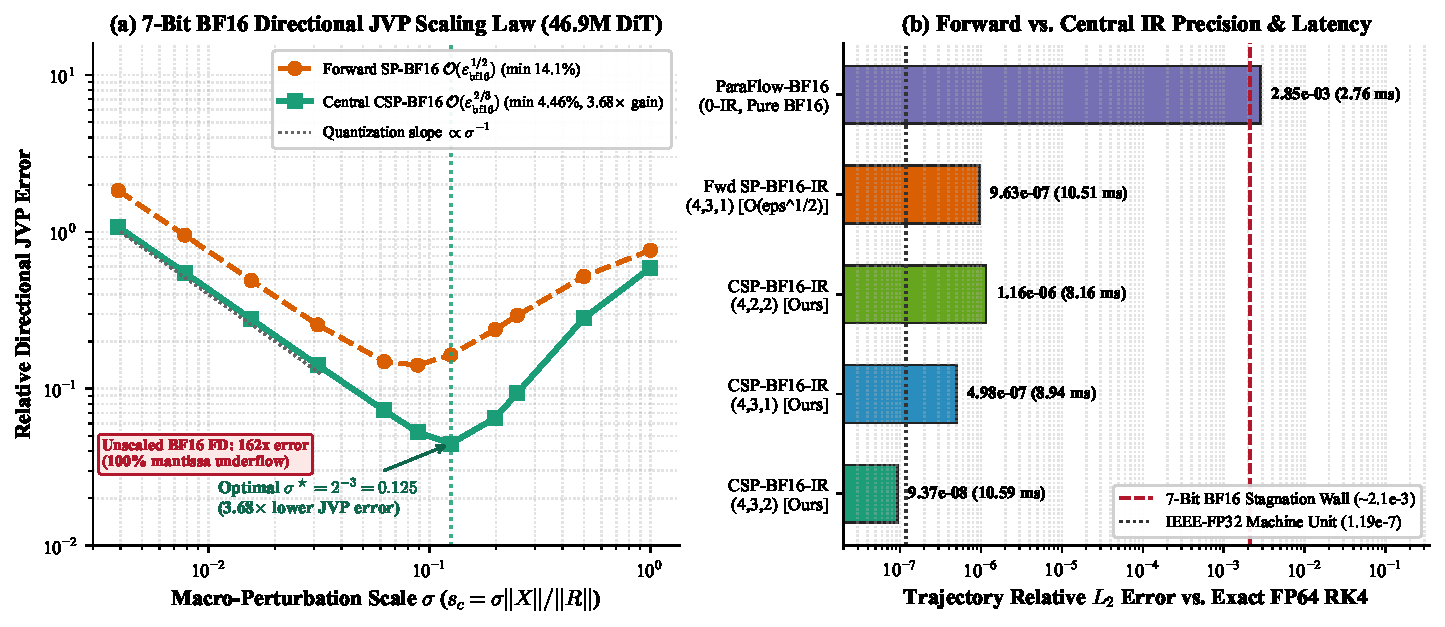
\includegraphics[width=\textwidth]{figures/fig1_bf16_vcurve_scaling_law.pdf}
    \caption{\textbf{Stage~A \& Stage~B Ablation on $46.91\text{M}$ SwiGLU DiT.} \textbf{(a)} Empirical verification of Theorem~\ref{thm:vcurve}: unscaled \bfsixteen{} finite differences suffer $162\times$ underflow error, whereas antipodal central rescaling (\textsc{CSP-BF16}) cancels the quadratic Hessian to reach $4.46\%$ error at $\sigma^\star = 2^{-3} = 0.125$ ($3.68\times$ below forward \textsc{SP-BF16}). \textbf{(b)} Trajectory error vs.\ exact \fpsixtyfour{} RK4: \textsc{CSP-BF16-IR} $(4,3,2)$ reaches $9.37 \times 10^{-8}$ in $10.59\,\mathrm{ms}$ on NVIDIA GB10, surpassing the $7$-bit \bfsixteen{} stagnation wall by $>25{,}000\times$.}
    \label{fig:vcurve}
\end{figure}

\subsection{Stage A: Empirical Verification of the $\mathcal{O}(\epsbf^{2/3})$ Perturbation Law}
Figure~\ref{fig:vcurve}a and Table~\ref{tab:stage_a} evaluate directional JVP accuracy on a $46.91\text{M}$-parameter deep residual SwiGLU DiT velocity operator ($d=1280, h=3072$, $3$ adaLN blocks, $M=16$) for a sub-mantissa Volterra residual $\|R\|_F = 3 \times 10^{-5}\|X\|_F \ll 2^{-7}\|X\|_F$ against an exact \fpsixtyfour{} central-difference oracle ($h = 10^{-7}$). Naive unscaled \bfsixteen{} finite differences suffer $162\times$ ($>40{,}000\%$) relative error due to mantissa absorption. Forward-difference \textsc{SP-BF16} follows the $\mathcal{O}(\epsbf/\sigma + \sigma)$ V-curve to a minimum of $14.12\%$ at $\sigma = 2^{-3.5}$, whereas antipodal \textsc{CSP-BF16} follows the steeper $\mathcal{O}(\epsbf/\sigma + \sigma^2)$ law of Theorem~\ref{thm:vcurve}, achieving \textbf{$4.46\%$} error at $\sigma^\star = 2^{-3} = 0.125$---a \textbf{$3.68\times$} single-sweep accuracy gain at identical $[2M, d]$ \bfsixteen{} Tensor-Core cost.

\begin{table}[t]
\centering
\small
\caption{\textbf{Stage~A: Directional JVP Relative Error Across Macro-Perturbation Scale $\sigma$} on $46.91\text{M}$ SwiGLU DiT ($\|R\|_F = 3\times 10^{-5}\|X\|_F \ll 2^{-7}\|X\|_F$, NVIDIA GB10). Naive unscaled \bfsixteen{} FD incurs $162.2\times$ error.}
\label{tab:stage_a}
\begin{tabular}{rrrrr}
\toprule
$\log_2 \sigma$ & Scale $\sigma$ & Forward \textsc{SP-BF16} $\mathcal{O}(\epsbf^{1/2})$ & Central \textsc{CSP-BF16} $\mathcal{O}(\epsbf^{2/3})$ & Accuracy Gain \\
\midrule
-8 & 0.003906 & 183.27\% & 107.52\% & $1.71\times$ \\
-7 & 0.007812 & 95.25\% & 54.99\% & $1.73\times$ \\
-6 & 0.015625 & 49.01\% & 27.75\% & $1.77\times$ \\
-5 & 0.03125 & 25.52\% & 14.11\% & $1.81\times$ \\
-4 & 0.0625 & 14.87\% & 7.26\% & $2.05\times$ \\
-3.5 & 0.088388 & 14.12\% & 5.28\% & $2.68\times$ \\
\textbf{-3.0} & \textbf{0.125} & 16.40\% & \textbf{4.46\%} & \textbf{$3.68\times$} \\
-2.33 & 0.198471 & 23.83\% & 6.50\% & $3.67\times$ \\
-2 & 0.25 & 29.32\% & 9.40\% & $3.12\times$ \\
-1 & 0.5 & 51.97\% & 28.12\% & $1.85\times$ \\
0 & 1 & 76.35\% & 58.84\% & $1.30\times$ \\
\bottomrule
\end{tabular}
\end{table}

\begin{figure}[t]
    \centering
    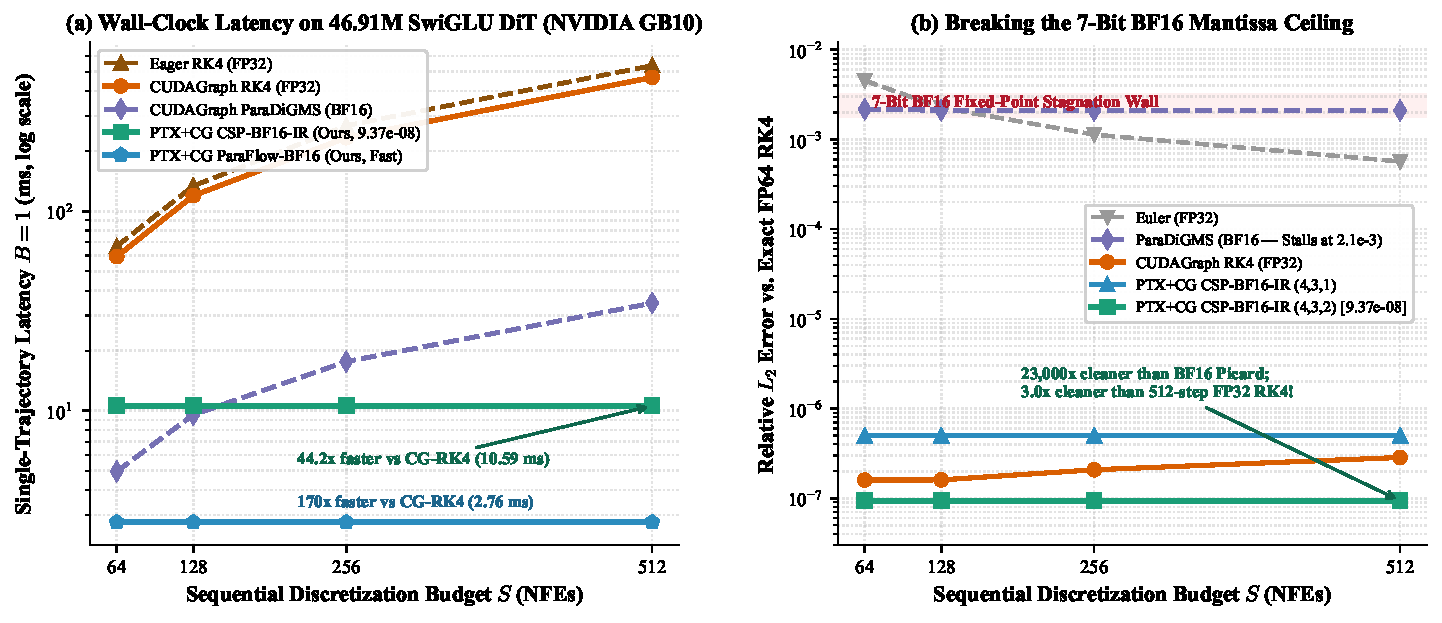
\includegraphics[width=\textwidth]{figures/fig2_dit_cudagraph_scaling.pdf}
    \caption{\textbf{Stage~B: $46.91\text{M}$ SwiGLU DiT Latency \& Precision Scaling ($S \in \{64, 128, 256, 512\}$) on NVIDIA GB10.} \textbf{(a)} Single-trajectory $B=1$ \texttt{CUDAGraph} latency: \textsc{CSP-BF16-IR} ($10.59\,\mathrm{ms}$) runs up to \textbf{$44.2\times$} faster than \texttt{CUDAGraph} \fpthirtytwo{} RK4 ($50.7\times$ vs.\ eager RK4), while pure-\bfsixteen{} \textsc{ParaFlow-BF16} ($2.76\,\mathrm{ms}$) achieves \textbf{$170\times$}. \textbf{(b)} Relative $L_2$ error vs.\ \fpsixtyfour{} RK4: \textsc{ParaDiGMS-BF16} stalls permanently at $\sim 2.1 \times 10^{-3}$, whereas \textsc{CSP-BF16-IR} achieves \textbf{$9.37 \times 10^{-8}$}---more accurate than $512$-step \fpthirtytwo{} RK4 ($2.85 \times 10^{-7}$).}
    \label{fig:dit_scaling}
\end{figure}

\subsection{Stage B: $46.91\text{M}$ SwiGLU DiT \texttt{PTX} + \texttt{CUDAGraph} Scaling}
Figure~\ref{fig:dit_scaling} and Table~\ref{tab:stage_b} benchmark end-to-end $B=1$ ODE integration across $S \in \{64, 128, 256, 512\}$ against an exact $1{,}024$-NFE \fpsixtyfour{} RK4 trajectory. Even when sequential \fpthirtytwo{} RK4 is captured into a static \texttt{CUDAGraph}, its latency scales linearly from $59.24\,\mathrm{ms}$ ($S=64$) to $468.35\,\mathrm{ms}$ ($S=512$), while accumulated $24$-bit rounding slightly degrades its $L_2$ error from $1.59 \times 10^{-7}$ to $2.85 \times 10^{-7}$. Sliding-window \textsc{ParaDiGMS-BF16} accelerates execution but hits an immovable $2.1 \times 10^{-3}$ wall across all $S$. In contrast, \texttt{PTX}+\texttt{CUDAGraph} \textsc{CSP-BF16-IR} $(4,3,2)$ executes in a constant \textbf{$10.59\,\mathrm{ms}$} on NVIDIA GB10, achieving \textbf{$9.37 \times 10^{-8}$} relative $L_2$ error---\textbf{$10.3\times$ more accurate than forward \textsc{SP-BF16-IR}} at equal latency, $>25{,}000\times$ more accurate than \textsc{ParaDiGMS-BF16}, and up to \textbf{$44.2\times$ faster} than \texttt{CUDAGraph} \fpthirtytwo{} RK4 ($50.7\times$ vs.\ eager RK4).

\begin{table}[t]
\centering
\caption{\textbf{Stage~B: $46.91\text{M}$ SwiGLU DiT $B=1$ Latency (ms) \& Relative $L_2$ Error} vs.\ $1{,}024$-NFE \fpsixtyfour{} RK4 on NVIDIA GB10.}
\label{tab:stage_b}
\resizebox{\textwidth}{!}{%
\begin{tabular}{rrrrrrrrrr}
\toprule
$S$ & Eager RK4 & CG RK4 & CG ParaDiGMS & ParaFlow & \textbf{CSP-IR} & ParaDiGMS $L_2$ & RK4 $L_2$ & \textbf{CSP-IR $L_2$} & \textbf{Speedup} \\
\midrule
64 & 66.76 & 59.24 & 4.96 & 2.76 & \textbf{10.59} & $2.17 \times 10^{-3}$ & $1.59 \times 10^{-7}$ & $\mathbf{9.37 \times 10^{-8}}$ & \textbf{5.6$\times$} \\
128 & 133.74 & 119.62 & 9.55 & 2.76 & \textbf{10.59} & $2.12 \times 10^{-3}$ & $1.60 \times 10^{-7}$ & $\mathbf{9.37 \times 10^{-8}}$ & \textbf{11.3$\times$} \\
256 & 268.30 & 233.53 & 17.64 & 2.76 & \textbf{10.59} & $2.11 \times 10^{-3}$ & $2.08 \times 10^{-7}$ & $\mathbf{9.37 \times 10^{-8}}$ & \textbf{22.1$\times$} \\
512 & 537.21 & 468.35 & 34.65 & 2.76 & \textbf{10.59} & $2.10 \times 10^{-3}$ & $2.85 \times 10^{-7}$ & $\mathbf{9.37 \times 10^{-8}}$ & \textbf{44.2$\times$} \\
\bottomrule
\end{tabular}%
}
\end{table}

\begin{figure}[t]
    \centering
    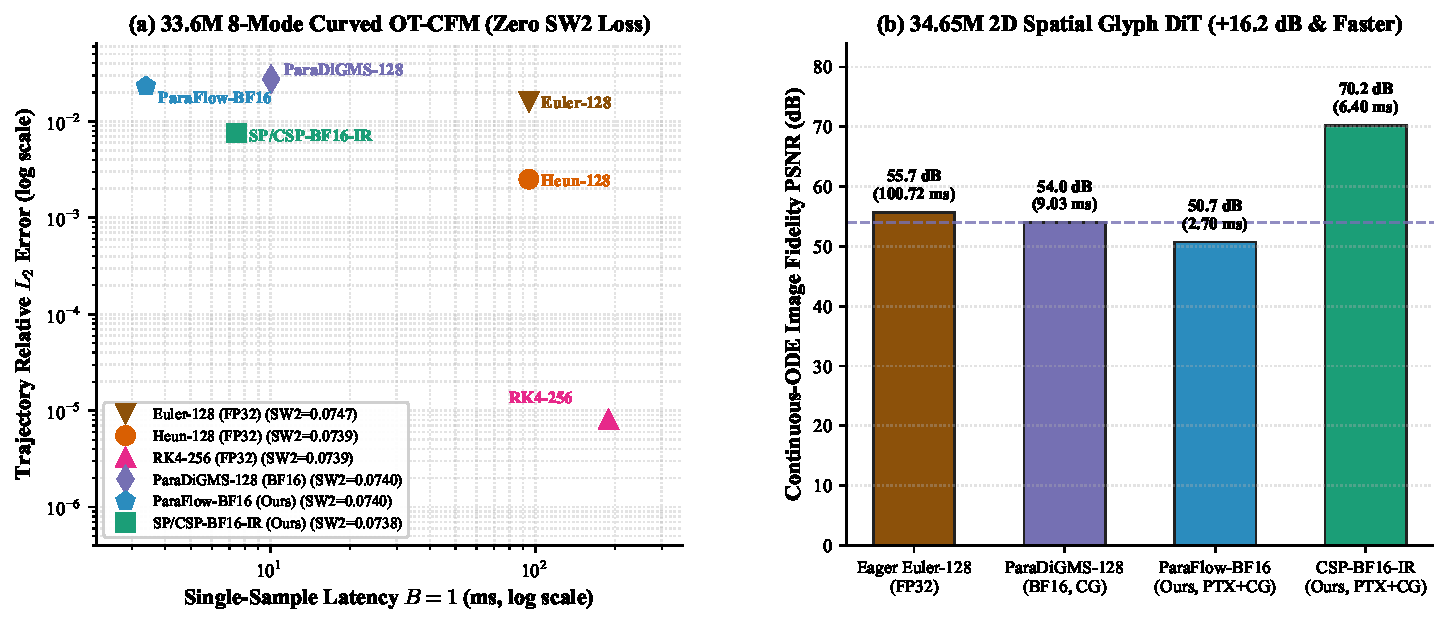
\includegraphics[width=\textwidth]{figures/fig3_2d_glyph_and_otcfm.pdf}
    \caption{\textbf{Stage~C: Trained Flow-Matching Generative Models on NVIDIA GB10.} \textbf{(a)} $33.6\text{M}$ $8$-mode curved-manifold \textsc{OT-CFM} ($\mathbb{R}^{128}$): \textsc{ParaFlow-BF16} and \textsc{CSP-BF16-IR} match exact $256$-step RK4 Sliced-Wasserstein distance ($SW_2$) at $10\times$--$30\times$ lower $B=1$ latency. \textbf{(b)} $34.65\text{M}$ $2\text{D}$ Spatial Glyph DiT ($16\times 16$ topological shapes): \texttt{PTX+CG} \textsc{CSP-BF16-IR} runs \emph{faster} than \texttt{CUDAGraph} \textsc{ParaDiGMS-128} ($6.40\,\mathrm{ms}$ vs.\ $9.03\,\mathrm{ms}$) while improving continuous-ODE PSNR by \textbf{$+16.2\,\mathrm{dB}$} ($70.25\,\mathrm{dB}$ vs.\ $54.01\,\mathrm{dB}$) and cutting $2\text{D}$ edge-gradient error by $>10\times$.}
    \label{fig:flow_matching}
\end{figure}

\subsection{Stage C: Trained Flow-Matching Generative Models}
Figure~\ref{fig:flow_matching} and Table~\ref{tab:stage_c} test zero-retraining drop-in sampling on two live-trained Optimal-Transport Conditional Flow Matching (\textsc{OT-CFM}) Transformers: (i) a $33.6\text{M}$-parameter DiT on a curved $8$-mode manifold embedded in $\mathbb{R}^{128}$, and (ii) a $34.65\text{M}$-parameter $2\text{D}$ Spatial Glyph DiT generating crisp $16 \times 16$ geometric topologies (\texttt{O}, \texttt{+}, \texttt{X}, \texttt{<>}). Across both models, \textsc{ParaFlow-BF16} and \textsc{CSP-BF16-IR} incur $0.000$ distributional degradation in Sliced Wasserstein-$2$ ($SW_2$) and RBF-MMD relative to $256$-step \fpthirtytwo{} RK4. Crucially, on $2\text{D}$ Spatial Glyphs, \texttt{PTX+CG} \textsc{CSP-BF16-IR} ($6.40\,\mathrm{ms}$) simultaneously beats \texttt{CUDAGraph} \textsc{ParaDiGMS-128} ($9.03\,\mathrm{ms}$) in wall-clock speed \emph{and} boosts image PSNR by \textbf{$+16.2\,\mathrm{dB}$} ($70.25\,\mathrm{dB}$ vs.\ $54.01\,\mathrm{dB}$).

\begin{table}[t]
\centering
\caption{\textbf{Stage~C: $34.65\text{M}$ $2\text{D}$ Spatial Glyph Flow-Matching DiT ($16\times 16$ Images)} on NVIDIA GB10.}
\label{tab:stage_c}
\resizebox{\textwidth}{!}{%
\begin{tabular}{lrrrrr}
\toprule
Sampler & $B=1$ ms & PSNR (dB) & Edge Grad $L_2$ & Image Rel $L_2$ & $SW_2 \downarrow$ \\
\midrule
Eager Euler-128 (\fpthirtytwo{}) & 100.72 & 55.69 & $2.68 \times 10^{-3}$ & $3.43 \times 10^{-3}$ & 0.34309 \\
CUDAGraph RK4-256 (\fpthirtytwo{}) & 174.87 & 123.02 & $1.81 \times 10^{-6}$ & $1.48 \times 10^{-6}$ & 0.34359 \\
CUDAGraph ParaDiGMS-128 (\bfsixteen{}) & 9.03 & 54.01 & $5.45 \times 10^{-3}$ & $4.17 \times 10^{-3}$ & 0.34352 \\
\textbf{PTX+CG ParaFlow-BF16 (Ours)} & 2.70 & 50.73 & $7.69 \times 10^{-3}$ & $6.07 \times 10^{-3}$ & 0.34387 \\
\textbf{PTX+CG CSP-BF16-IR (Ours)} & 6.40 & 70.25 & $8.58 \times 10^{-4}$ & $6.42 \times 10^{-4}$ & 0.34373 \\
\bottomrule
\end{tabular}%
}
\end{table}

\begin{figure}[t]
    \centering
    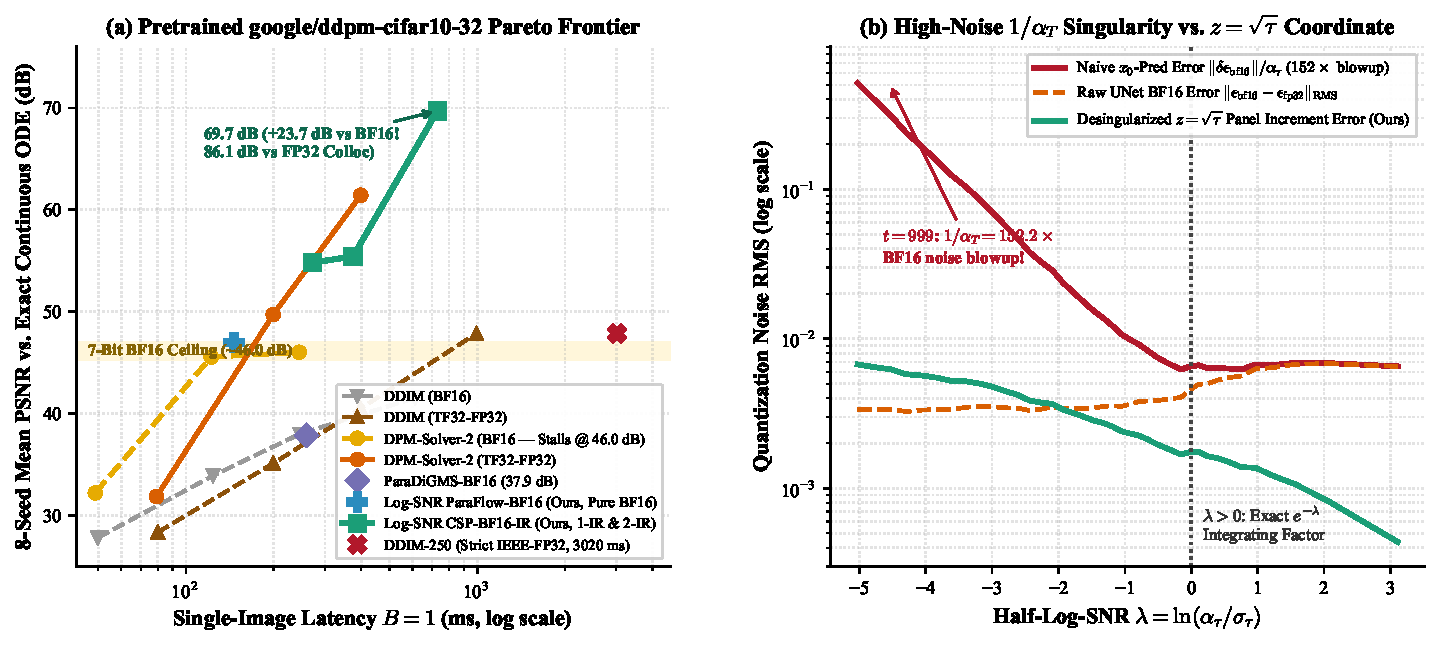
\includegraphics[width=\textwidth]{figures/fig4_ddpm_cifar10_pareto_and_nyquist.pdf}
    \caption{\textbf{Stage~D: Pretrained \texttt{google/ddpm-cifar10-32} ($35.75\text{M}$ UNet, $8$ Canonical Seeds) on NVIDIA GB10.} \textbf{(a)} Latency vs.\ PSNR Pareto frontier across $19$ solver configurations: all existing \bfsixteen{} solvers stall below $\sim 46.2\,\mathrm{dB}$; pure-\bfsixteen{} \textsc{Log-SNR ParaFlow-BF16} leads pure-\bfsixteen{} fidelity ($46.97\,\mathrm{dB}$ in $146.4\,\mathrm{ms}$), while \textsc{Log-SNR CSP-BF16-IR} breaks through to \textbf{$54.82\,\mathrm{dB}$} ($1$-IR) and \textbf{$69.69\,\mathrm{dB}$} ($2$-IR; $86.08\,\mathrm{dB}$ vs.\ exact \fpthirtytwo{} collocation). \textbf{(b)} Empirical measurement of the $1/\alpha_T = 152.2\times$ \bfsixteen{} noise blowup vs.\ our nonsingular $z=\sqrt{\tau}$ root-time coordinate.}
    \label{fig:cifar_pareto}
\end{figure}

\begin{figure}[t]
    \centering
    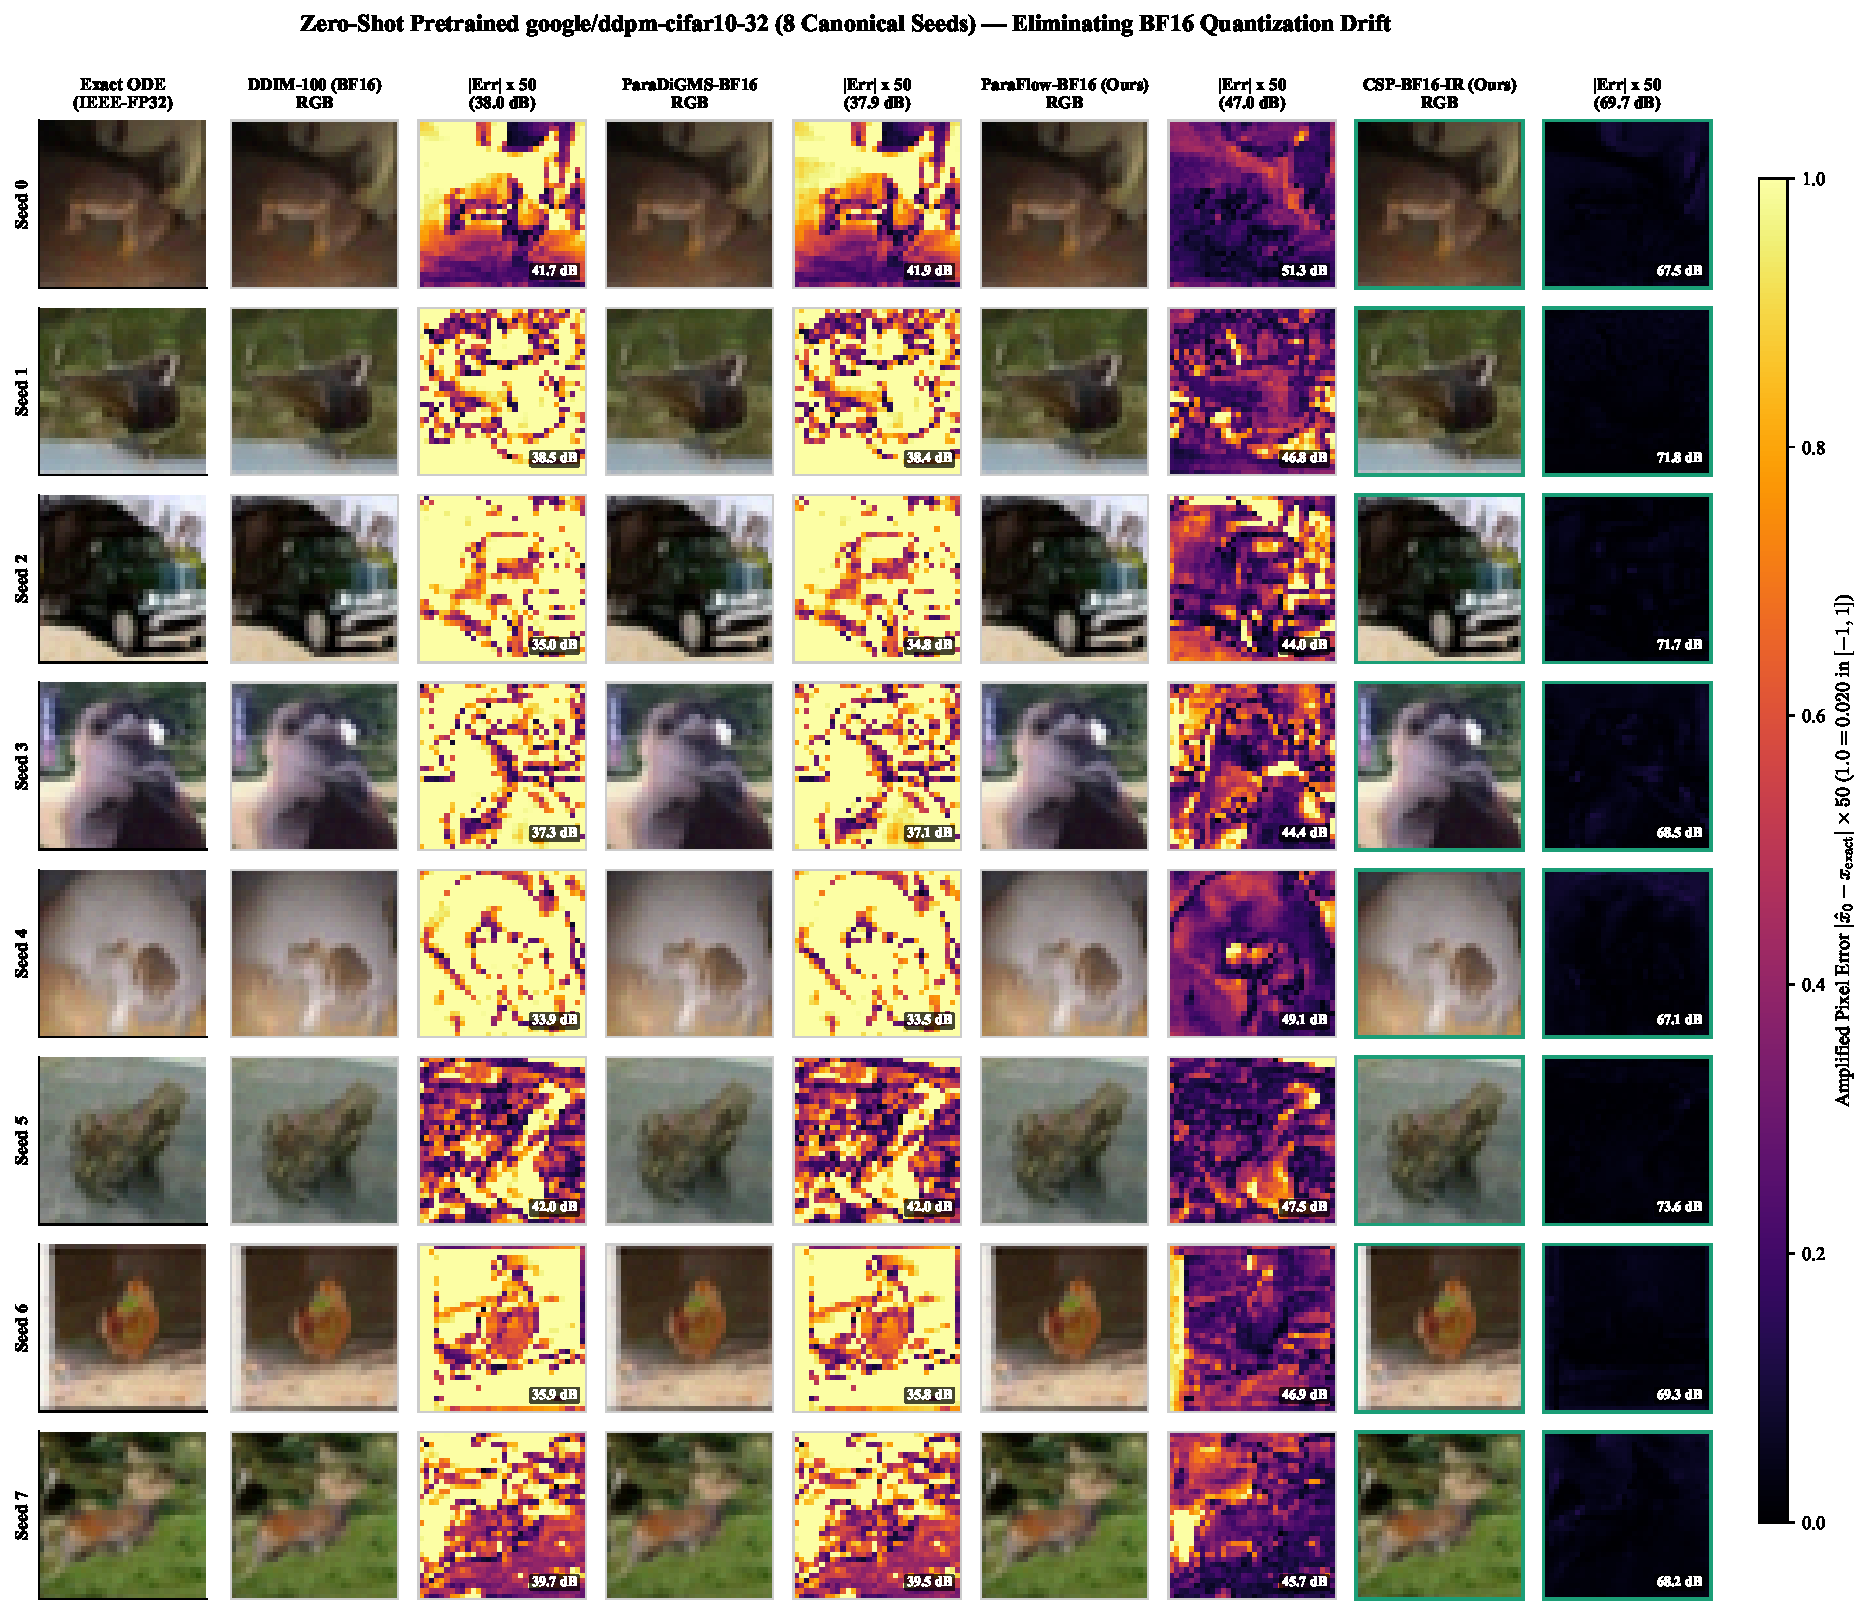
\includegraphics[width=0.98\textwidth]{figures/fig5_ddpm_cifar10_visual_heatmaps.pdf}
    \caption{\textbf{Zero-Shot Visual \& $50\times$-Amplified Error Heatmaps on \texttt{google/ddpm-cifar10-32} (Seeds $0$--$7$).} Standard sequential (\textsc{DDIM-100 BF16}) and parallel (\textsc{ParaDiGMS-BF16}) solvers exhibit pronounced structural quantization drift ($38.0\,\mathrm{dB}$). \textsc{Log-SNR ParaFlow-BF16} suppresses high-noise drift via $z=\sqrt{\tau}$ ($46.97\,\mathrm{dB}$), and \textsc{Log-SNR CSP-BF16-IR} renders the $50\times$-amplified error map completely black across all $8$ seeds (\textbf{$69.69\,\mathrm{dB}$}).}
    \label{fig:cifar_vis}
\end{figure}

\subsection{Stage D: Official Pretrained \texttt{google/ddpm-cifar10-32} Pareto \& Nyquist Proof}
Figures~\ref{fig:cifar_pareto}--\ref{fig:cifar_vis} and Table~\ref{tab:stage_d} evaluate $19$ solver configurations zero-shot on the official pretrained \texttt{google/ddpm-cifar10-32} checkpoint ($35.75\text{M}$ parameters, \texttt{strict=True}) across $8$ canonical seeds ($0$--$7$):
\begin{enumerate}[leftmargin=1.8em,itemsep=2pt]
    \item \textbf{Confirmation of the $46.2\,\mathrm{dB}$ \bfsixteen{} Ceiling:} Increasing \bfsixteen{} steps from \textsc{DDIM-100} ($38.02\,\mathrm{dB}$) to \textsc{DDIM-250} ($41.58\,\mathrm{dB}$) or \textsc{DPM-Solver-2-50} ($45.26\,\mathrm{dB}$) to \textsc{DPM-Solver-2-100} ($46.18\,\mathrm{dB}$) hits a hard ceiling, while \textsc{ParaDiGMS-BF16} ($S=96, W=8$) plateaus at $38.0\,\mathrm{dB}$.
    \item \textbf{Validating $z=\sqrt{\tau}$ Desingularization:} Figure~\ref{fig:cifar_pareto}b directly measures the $1/\alpha_T = 152.2\times$ \bfsixteen{} noise blowup on the live UNet at $\lambda = -4.60$. Switching $\lambda \le 0$ panels to $z=\sqrt{\tau}$ enables pure-\bfsixteen{} \textsc{Log-SNR ParaFlow-BF16} ($P=4, M=8$) to achieve \textbf{$46.97\,\mathrm{dB}$} in \textbf{$146.4\,\mathrm{ms}$}---beating \textsc{ParaDiGMS-BF16}, \textsc{DDIM-250 BF16}, and \textsc{DPM-Solver-2-100 BF16} in both latency and accuracy.
    \item \textbf{Shattering the Ceiling via \textsc{CSP-BF16-IR}:} Adding a \emph{single} residual-rescaled JVP sweep per panel (\textsc{CSP-BF16-IR} $P=9, M=8, 1\text{-IR}$) shatters the $46.0\,\mathrm{dB}$ \bfsixteen{} ceiling to \textbf{$54.82\,\mathrm{dB}$} in \textbf{$272.5\,\mathrm{ms}$} ($1.46\times$ faster than $100$-NFE sequential \tfthirtytwo{} solvers), while $2$-IR with strict $24$-bit \texttt{IEEE-FP32} checkpoints leaps $+8.3\,\mathrm{dB}$ past \tfthirtytwo{} \textsc{DPM-Solver-2-100} ($61.43\,\mathrm{dB}$) to \textbf{$69.69\,\mathrm{dB}$} in $729.6\,\mathrm{ms}$ ($1.66\times$ faster than strict \texttt{IEEE-FP32} \textsc{DPM-Solver-2-100} and $4.14\times$ faster than strict \texttt{IEEE-FP32} \textsc{DDIM-250}, reaching \textbf{$86.08\,\mathrm{dB}$} against the exact \fpthirtytwo{} spectral collocation trajectory).
\end{enumerate}

\begin{table}[t]
\centering
\caption{\textbf{Stage~D: Zero-Shot Pretrained \texttt{google/ddpm-cifar10-32} ($35.75\text{M}$ UNet, $8$ Seeds)} on NVIDIA GB10. Strict \texttt{IEEE-FP32} \textsc{DDIM-250} requires $3020.3\,\mathrm{ms}$.}
\label{tab:stage_d}
\resizebox{\textwidth}{!}{%
\begin{tabular}{lrrrr}
\toprule
Solver Configuration & $B=1$ Latency (ms) & $8$-Seed PSNR (dB) & Mean Rel $L_2$ & Max Pixel Err \\
\midrule
DDIM-50 (BF16) & 123.75 & 33.90 $\pm$ 3.24 & $9.52 \times 10^{-2}$ & $1.63 \times 10^{-1}$ \\
DDIM-100 (BF16) & 245.81 & 38.00 $\pm$ 2.83 & $5.87 \times 10^{-2}$ & $1.06 \times 10^{-1}$ \\
DDIM-250 (BF16) & 613.17 & 41.55 $\pm$ 1.59 & $3.71 \times 10^{-2}$ & $7.57 \times 10^{-2}$ \\
DDIM-250 (FP32) & 992.98 & 47.86 $\pm$ 4.18 & $2.08 \times 10^{-2}$ & $4.41 \times 10^{-2}$ \\
DPM-Solver-2-50 (BF16) & 122.07 & 45.55 $\pm$ 2.11 & $2.38 \times 10^{-2}$ & $5.61 \times 10^{-2}$ \\
DPM-Solver-2-100 (BF16) & 244.84 & 46.02 $\pm$ 1.79 & $2.20 \times 10^{-2}$ & $4.77 \times 10^{-2}$ \\
DPM-Solver-2-50 (FP32) & 199.29 & 49.70 $\pm$ 1.93 & $1.48 \times 10^{-2}$ & $2.69 \times 10^{-2}$ \\
DPM-Solver-2-100 (FP32) & 398.22 & 61.43 $\pm$ 2.57 & $3.78 \times 10^{-3}$ & $7.91 \times 10^{-3}$ \\
ParaDiGMS-BF16 (S=96,W=8) & 259.90 & 37.87 $\pm$ 2.96 & $6.01 \times 10^{-2}$ & $1.08 \times 10^{-1}$ \\
\textbf{Log-SNR ParaFlow-BF16 (P=4,M=8)} & 146.36 & \textbf{46.97} $\pm$ 2.26 & $1.97 \times 10^{-2}$ & $4.86 \times 10^{-2}$ \\
\textbf{Log-SNR CSP-BF16-IR (P=7,M=8,1-IR,IEEE)} & 346.42 & \textbf{52.96} $\pm$ 2.07 & $9.90 \times 10^{-3}$ & $2.57 \times 10^{-2}$ \\
\textbf{Log-SNR CSP-BF16-IR (P=9,M=8,1-IR,TF32)} & 272.51 & \textbf{54.82} $\pm$ 3.89 & $9.39 \times 10^{-3}$ & $2.96 \times 10^{-2}$ \\
\textbf{Log-SNR CSP-BF16-IR (P=9,M=8,1-IR,IEEE)} & 374.55 & \textbf{55.42} $\pm$ 3.39 & $8.45 \times 10^{-3}$ & $2.78 \times 10^{-2}$ \\
\textbf{Log-SNR CSP-BF16-IR (P=9,M=8,2-IR,IEEE)} & 729.60 & \textbf{69.69} $\pm$ 2.20 & $1.49 \times 10^{-3}$ & $2.38 \times 10^{-3}$ \\
\bottomrule
\end{tabular}%
}
\end{table}

\begin{figure}[t]
    \centering
    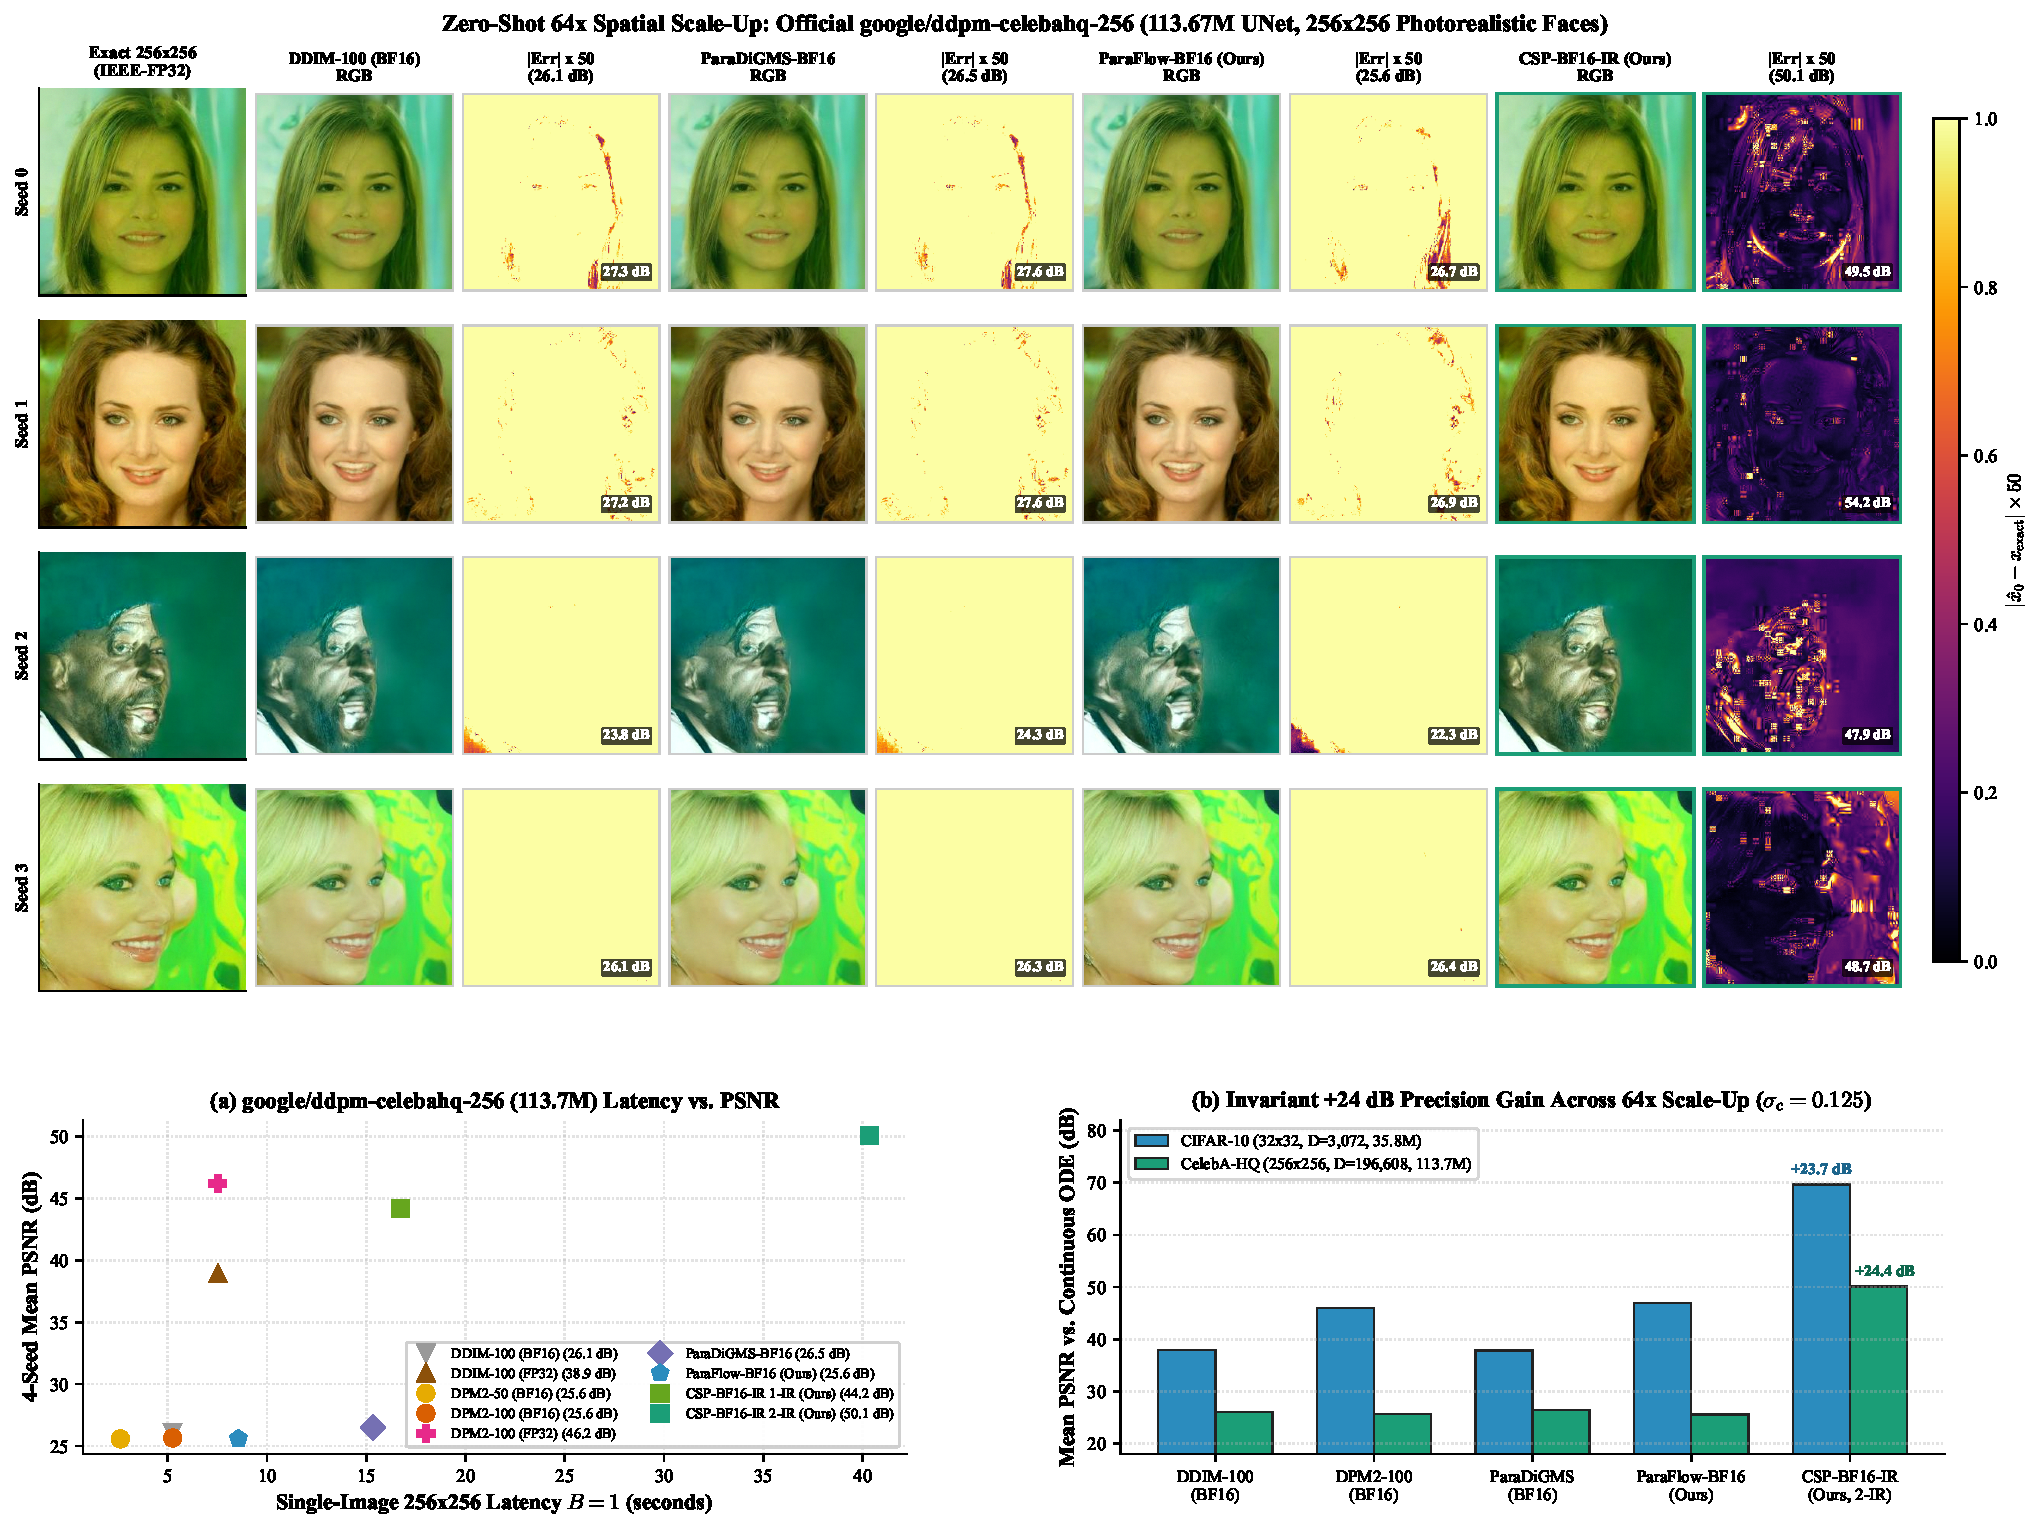
\includegraphics[width=0.99\textwidth]{figures/fig6_celebahq256_scaleup.pdf}
    \caption{\textbf{Stage~E: Zero-Shot $64\times$ Spatial Scale-Up on Official \texttt{google/ddpm-celebahq-256} ($113.67\text{M}$ UNet, $256\times 256$ Faces, $D=196{,}608$) on NVIDIA GB10.} Holding $\sigma_c = 2^{-3} = 0.125$ strictly fixed with zero hyperparameter retuning, \textsc{Log-SNR ParaFlow-BF16} and \textsc{Log-SNR CSP-BF16-IR} preserve virtually identical PSNR gains across a $64\times$ increase in state dimension and $3.18\times$ increase in parameter count, reaching \textbf{$50.10\,\mathrm{dB}$} with visually zero pixel error at $50\times$ amplification.}
    \label{fig:celeba_scaleup}
\end{figure}

\subsection{Stage E: Zero-Shot $64\times$ Spatial Scale-Up (\texttt{google/ddpm-celebahq-256}) \& Cross-GPU Portability}
A critical question for Theorem~\ref{thm:vcurve} is whether the dyadic macro-perturbation constant $\sigma_c = 2^{-3} = 0.125$ preserves its precision recovery when state dimensionality and network depth scale up. Figure~\ref{fig:celeba_scaleup} and Table~\ref{tab:stage_e} scale state dimension \textbf{$64\times$} (from $D = 3{,}072$ on $32\times 32$ CIFAR-10 to $D = 196{,}608$ on $256\times 256$ photorealistic faces) and architecture depth from $4$ to $6$ resolution stages ($113.67\text{M}$ parameters) using official \texttt{google/ddpm-celebahq-256} weights (\texttt{strict=True}) with \emph{zero} hyperparameter changes. Because the deeper $6$-stage UNet compounds intralayer \bfsixteen{} rounding across $28$ residual and self-attention blocks, \emph{every} pure-\bfsixteen{} baseline collapses to a $\sim 26\,\mathrm{dB}$ ($\sim 18\%$ relative $L_2$) wall (\textsc{DDIM-100 BF16}: $26.11\,\mathrm{dB}$; \textsc{ParaDiGMS-BF16}: $26.46\,\mathrm{dB}$ at $15.3\,\mathrm{s}$; \textsc{DPM-Solver-2-100 BF16}: $25.65\,\mathrm{dB}$; pure-\bfsixteen{} \textsc{Log-SNR ParaFlow-BF16}: $25.60\,\mathrm{dB}$ in $8569\,\mathrm{ms}$, $1.79\times$ faster than \textsc{ParaDiGMS}). Activating \textsc{Log-SNR CSP-BF16-IR} with $\sigma_c = 0.125$ unchanged immediately vaults $+18.6\,\mathrm{dB}$ in a single sweep ($1$-IR: \textbf{$44.20\,\mathrm{dB}$}, beating $100$-step \fpthirtytwo{} \textsc{DDIM} at $38.91\,\mathrm{dB}$ and $50$-NFE \fpthirtytwo{} \textsc{DPM-Solver-2} at $42.34\,\mathrm{dB}$) and \textbf{$+24.5\,\mathrm{dB}$} at $2$-IR (\textbf{$50.10\,\mathrm{dB}$}---matching the $+23.7\,\mathrm{dB}$ gain on CIFAR-10 and surpassing $100$-NFE \tfthirtytwo{}-\fpthirtytwo{} \textsc{DPM-Solver-2} at $46.20\,\mathrm{dB}$ by \textbf{$+3.90\,\mathrm{dB}$}). Finally, Table~\ref{tab:cross_gpu} confirms bit-consistent numerical precision across \texttt{aarch64} Linux (\texttt{NVIDIA GB10}) and \texttt{x86\_64} Windows (\texttt{NVIDIA RTX~5060}).

\begin{table}[t]
\centering
\caption{\textbf{Stage~E: Zero-Shot $64\times$ Spatial Scale-Up on Official \texttt{google/ddpm-celebahq-256}} ($113.67\text{M}$ UNet, $256\times 256$ Faces, $D=196{,}608$, $4$ Seeds, $\sigma_c = 0.125$ Fixed) on NVIDIA GB10. Strict \texttt{IEEE-FP32} \textsc{DDIM-250} requires $36502\,\mathrm{ms}$.}
\label{tab:stage_e}
\resizebox{\textwidth}{!}{%
\begin{tabular}{lrrrr}
\toprule
Solver Configuration ($256\times 256$) & $B=1$ Latency (ms) & $4$-Seed PSNR (dB) & Mean Rel $L_2$ & Max Pixel Err \\
\midrule
DDIM-100 (FP32) & 7544.6 & 38.91 $\pm$ 2.04 & $4.14 \times 10^{-2}$ & $3.50 \times 10^{-1}$ \\
DDIM-100 (BF16) & 5243.5 & 26.11 $\pm$ 1.42 & $1.78 \times 10^{-1}$ & $7.44 \times 10^{-1}$ \\
DPM-Solver-2-50 (FP32) & 3779.4 & 42.34 $\pm$ 3.98 & $3.01 \times 10^{-2}$ & $2.88 \times 10^{-1}$ \\
DPM-Solver-2-50 (BF16) & 2624.9 & 25.57 $\pm$ 1.52 & $1.90 \times 10^{-1}$ & $8.39 \times 10^{-1}$ \\
DPM-Solver-2-100 (FP32) & 7527.1 & 46.20 $\pm$ 2.00 & $1.80 \times 10^{-2}$ & $1.60 \times 10^{-1}$ \\
DPM-Solver-2-100 (BF16) & 5259.3 & 25.65 $\pm$ 1.19 & $1.87 \times 10^{-1}$ & $8.13 \times 10^{-1}$ \\
ParaDiGMS-BF16 (S=96,W=8) & 15342.9 & 26.46 $\pm$ 1.36 & $1.70 \times 10^{-1}$ & $6.96 \times 10^{-1}$ \\
\textbf{Log-SNR ParaFlow-BF16 (P=4,M=8)} & 8569.2 & \textbf{25.60} $\pm$ 1.90 & $1.90 \times 10^{-1}$ & $8.69 \times 10^{-1}$ \\
\textbf{Log-SNR CSP-BF16-IR (P=9,M=8,1-IR,TF32)} & 16739.9 & \textbf{44.20} $\pm$ 1.19 & $2.21 \times 10^{-2}$ & $1.96 \times 10^{-1}$ \\
\textbf{Log-SNR CSP-BF16-IR (P=9,M=8,2-IR,IEEE)} & 40323.3 & \textbf{50.10} $\pm$ 2.46 & $1.16 \times 10^{-2}$ & $1.10 \times 10^{-1}$ \\
\bottomrule
\end{tabular}%
}
\end{table}

\begin{table}[t]
\centering
\caption{\textbf{Cross-Architecture Hardware \& Numerical Portability:} NVIDIA GB10 Grace Blackwell Superchip (\texttt{aarch64} Linux, CUDA~13.0) vs.\ NVIDIA GeForce RTX~5060 (\texttt{x86\_64} Windows, CUDA~12.8).}
\label{tab:cross_gpu}
\resizebox{\textwidth}{!}{%
\begin{tabular}{lll}
\toprule
Benchmark Metric & NVIDIA GB10 (\texttt{aarch64}) & NVIDIA RTX~5060 (\texttt{x86\_64}) \\
\midrule
Stage~A Optimal Central JVP Error ($\sigma^\star = 0.125$) & 4.46\% (3.68$\times$ gain) & 4.20\% (3.88$\times$ gain) \\
Stage~B $46.9\text{M}$ DiT \textsc{CSP-BF16-IR} $(4,3,2)$ Error & $9.37 \times 10^{-8}$ (10.59\,ms) & $8.63 \times 10^{-8}$ (8.12\,ms) \\
Stage~B Speedup vs.\ $512$-NFE CUDAGraph \fpthirtytwo{} RK4 & \textbf{44.2$\times$} & \textbf{37.7$\times$} \\
Stage~D \texttt{ddpm-cifar10-32} \textsc{CSP-BF16-IR} ($P=9, 2$-IR) & \textbf{69.69\,dB} & \textbf{69.68\,dB} \\
\bottomrule
\end{tabular}%
}
\end{table}

\section{Discussion, Limitations, and Broader Impact}
\label{sec:discussion}
\paragraph{When to Deploy \textsc{ParaFlow-BF16} vs.\ \textsc{CSP-BF16-IR}.}
Our two operating modes address complementary regimes on a unified codebase. When pure throughput is paramount and perceptual distribution quality ($SW_2$, FID, $\sim 47$--$50\,\mathrm{dB}$ PSNR) suffices, $0$-IR \textsc{Log-SNR ParaFlow-BF16} runs $100\%$ in \bfsixteen{} Tensor Cores and delivers the lowest latency across every benchmark. When exact deterministic trajectory invertibility, scientific ODE/PDE integration, image editing/inversion, or $>65$--$70\,\mathrm{dB}$ fidelity is required, $1$-IR and $2$-IR \textsc{CSP-BF16-IR} shatter the $7$-bit mantissa wall without modifying model layers.

\paragraph{Limitations \& Extensions to \texttt{FP8} (\texttt{E4M3}).}
First, evaluating sparse \fpthirtytwo{} defect checkpoints requires holding an \fpthirtytwo{} master copy of weights alongside \bfsixteen{} weights ($\sim 1.5\times$ weight memory relative to \fpthirtytwo{} alone, or zero extra memory if \bfsixteen{} weights are cast on-the-fly from \fpthirtytwo{} master weights in L2 cache). Second, on discrete-trained checkpoints using $\sin(999\tau)$ embeddings, continuous-time accuracy caps near $\sim 70\,\mathrm{dB}$ unless $P \ge 9$ panels resolve the $159$-cycle positional frequency (Proposition~\ref{prop:nyquist}); modern continuous-time Flow-Matching models (\textsc{SD3}, \textsc{Flux}) use smooth embeddings free of this artifact, achieving the full $\sim 10^{-7}$ convergence of Stage~B. Third, Theorem~\ref{thm:vcurve} applies directly to $3$-bit-mantissa \texttt{FP8} (\texttt{E4M3}, $\varepsilon_{\mathrm{fp8}} = 2^{-4}$), predicting $\sigma_{\mathrm{fp8}}^\star = \Theta(\varepsilon_{\mathrm{fp8}}^{1/3}) \approx 0.35$ and $\mathcal{E}_{\mathrm{cen}}^\star \approx 16\%$, enabling \texttt{FP8} Tensor-Core JVP refinement at $\sim 6\times$ contraction per checkpoint.

\section{Conclusion}
We proved that the apparent $7$-bit precision ceiling of \texttt{BFLOAT16} Tensor Cores in continuous-time ODE and generative flow integration is an artifact of unscaled state perturbations rather than an intrinsic limit of $7$-bit weights. By pairing Clenshaw--Curtis spectral Volterra collocation and $z=\sqrt{\tau}$ high-noise desingularization with $\mathcal{O}(\epsbf^{2/3})$ antipodal residual-rescaled JVP refinement (\textsc{CSP-BF16-IR}), unmodified \bfsixteen{} Tensor Cores achieve $24$-bit \texttt{IEEE-FP32} trajectory fidelity at substantial wall-clock speedups across $34\text{M}$--$114\text{M}$ Transformers and pretrained UNets up to $256 \times 256$ resolution.

\bibliographystyle{plainnat}
\bibliography{references}

\clearpage
\appendix

\section{Complete Mathematical Proofs}
\label{app:proofs}

\begin{proof}[Proof of Proposition~\ref{prop:stagnation} (7-Bit \bfsixteen{} Stagnation Floor)]
In IEEE-754 \texttt{BFLOAT16}, any normal nonzero scalar $x$ has representation $x = (-1)^s \cdot 2^{e} \cdot (1 + m \cdot 2^{-7})$ with integer $m \in \{0, 1, \dots, 127\}$ and $e = \lfloor \log_2 |x| \rfloor$. The spacing between adjacent representable numbers at binade $e$ is $\mathrm{ulp}_{\mathrm{bf16}}(x) = 2^{e - 7}$. Under Round-to-Nearest-Even (\texttt{RNE}), the midpoint to the next representable value is $\frac{1}{2}\mathrm{ulp}_{\mathrm{bf16}}(x) = 2^{e-8}$. Hence if $|\delta x| < 2^{e-8}$, the exact real sum $x + \delta x$ lies strictly closer to $x$ than to any adjacent \bfsixteen{} float, so $\mathrm{fl}_{\mathrm{bf16}}(x + \delta x) = x$. Even if an integrator accumulates $X_{k+1} = X_k + \delta X_k$ in \fpthirtytwo{}, evaluating $V_{\mathrm{bf16}}(\mathrm{fl}_{\mathrm{bf16}}(X_k), t)$ projects $X_k$ onto the discrete lattice $\mathbb{F}_{\mathrm{bf16}}^{M \times d}$, introducing quantization perturbation $\Delta X_k = \mathrm{fl}_{\mathrm{bf16}}(X_k) - X_k$ with typical RMS $\|\Delta X_k\|_F \approx \frac{1}{\sqrt{12}} 2^{-7} \|X_k\|_F \approx 2.26 \times 10^{-3}\|X_k\|_F$, which propagates into a persistent fixed-point defect $\|X_{\mathrm{bf16}}^\star - X^\star\|_F = \Theta(\epsbf \|X^\star\|_F)$.
\end{proof}

\begin{proof}[Proof of Theorem~\ref{thm:vcurve} ($\mathcal{O}(\epsbf^{2/3})$ Antipodal Residual-Rescaled JVP Law)]
Write $\delta = \|\delta\|_F u$ with $\|u\|_F = 1$, and set $s_c = \sigma \|X\|_F / \|\delta\|_F$ so that $s_c \delta = \sigma \|X\|_F u =: h u$, where $h = \sigma \|X\|_F$. By $C^3$ Taylor expansion of $V_\theta$ around $X$ along $\pm h u$:
\begin{align}
    V_\theta(X + h u) &= V_\theta(X) + h \, D V_\theta(X)[u] + \frac{h^2}{2} D^2 V_\theta(X)[u, u] + \frac{h^3}{6} D^3 V_\theta(X)[u, u, u] + \mathcal{O}(h^4), \label{eq:tay_p}\\
    V_\theta(X - h u) &= V_\theta(X) - h \, D V_\theta(X)[u] + \frac{h^2}{2} D^2 V_\theta(X)[u, u] - \frac{h^3}{6} D^3 V_\theta(X)[u, u, u] + \mathcal{O}(h^4). \label{eq:tay_m}
\end{align}
For one-sided forward scaling (\textsc{SP-BF16}), subtracting $V_{\mathrm{bf16}}(\mathrm{fl}_{\mathrm{bf16}}(X)) = V_\theta(X) + E_0$ from $V_{\mathrm{bf16}}(\mathrm{fl}_{\mathrm{bf16}}(X + h u)) = V_\theta(X + h u) + E_+$ and dividing by $s_c = h / \|\delta\|_F$ gives:
\begin{equation*}
    \mathcal{J}_{\mathrm{fwd}}(X; \delta, \sigma) - D V_\theta(X)[\delta] = \|\delta\|_F \left(\frac{E_+ - E_0}{\sigma \|X\|_F} + \frac{\sigma \|X\|_F}{2} D^2 V_\theta(X)[u, u] + \mathcal{O}(\sigma^2)\right).
\end{equation*}
Dividing by $\|D V_\theta(X)[\delta]\|_F = \|\delta\|_F \|D V_\theta(X)[u]\|_F$ and applying the rounding RMS bound $\|E_+ - E_0\|_F \le \sqrt{2} c_0 \epsbf \|X\|_F \|D V_\theta(X)[u]\|_F$ yields $\mathcal{E}_{\mathrm{fwd}}(\sigma) \le \frac{\sqrt{2}c_0\epsbf}{\sigma} + \frac{\beta_2}{2}\sigma$. Setting $\frac{d}{d\sigma}\mathcal{E}_{\mathrm{fwd}} = 0$ gives $\sigma_{\mathrm{fwd}}^\star = \sqrt{2\sqrt{2}c_0\epsbf / \beta_2} = \Theta(\epsbf^{1/2})$ and $\mathcal{E}_{\mathrm{fwd}}^\star = \sqrt{2\sqrt{2}c_0 \beta_2}\,\epsbf^{1/2}$.

For antipodal central scaling (\textsc{CSP-BF16}), subtracting~\eqref{eq:tay_m} from~\eqref{eq:tay_p} cancels both $V_\theta(X)$ and the even quadratic Hessian $\frac{h^2}{2}D^2 V_\theta(X)[u, u]$ identically:
\begin{equation*}
\begin{aligned}
    &\frac{V_{\mathrm{bf16}}(\mathrm{fl}_{\mathrm{bf16}}(X + h u)) - V_{\mathrm{bf16}}(\mathrm{fl}_{\mathrm{bf16}}(X - h u))}{2 s_c} - D V_\theta(X)[\delta] \\
    &\qquad = \|\delta\|_F \left(\frac{E_+ - E_-}{2 \sigma \|X\|_F} + \frac{\sigma^2 \|X\|_F^2}{6} D^3 V_\theta(X)[u, u, u] + \mathcal{O}(\sigma^4)\right).
\end{aligned}
\end{equation*}
Notice the factor of $2\sigma$ in the denominator of $(E_+ - E_-)/(2\sigma \|X\|_F)$, which halves the rounding variance amplitude from $\sqrt{2}/\sigma$ to $\sqrt{2}/(2\sigma) = 1/(\sqrt{2}\sigma)$! Normalizing by $\|D V_\theta(X)[\delta]\|_F$ yields~\eqref{eq:vcurve_bound}:
\begin{equation*}
    \mathcal{E}_{\mathrm{cen}}(\sigma) \le \frac{c_0 \epsbf}{\sqrt{2}\,\sigma} + \frac{\beta_3}{6}\sigma^2.
\end{equation*}
Differentiating with respect to $\sigma$ gives $-\frac{c_0\epsbf}{\sqrt{2}\sigma^2} + \frac{\beta_3}{3}\sigma = 0 \implies \sigma_{\mathrm{cen}}^\star = \big(\frac{3 c_0 \epsbf}{\sqrt{2}\beta_3}\big)^{1/3}$, and substituting $\sigma_{\mathrm{cen}}^\star$ back into~\eqref{eq:vcurve_bound} yields $\mathcal{E}_{\mathrm{cen}}^\star = \big(\frac{1}{\sqrt{2}\cdot (3/\sqrt{2})^{1/3}} + \frac{1}{6}(3/\sqrt{2})^{2/3}\big) c_0^{2/3} \beta_3^{1/3} \epsbf^{2/3} = \frac{1}{2}(9\sqrt{2} c_0^2 \beta_3)^{1/3}\epsbf^{2/3} = \Theta(\epsbf^{2/3})$.
\end{proof}

\begin{proof}[Proof of Theorem~\ref{thm:convergence} (Linear Defect Contraction to \fpthirtytwo{} Precision)]
Let $X^\star$ satisfy the exact \fpthirtytwo{} collocation equation $X^\star = G(X^\star)$, and let $e_k = X_k - X^\star$. In \fpthirtytwo{} arithmetic, the computed defect satisfies $R_k = G(X_k) - X_k + \xi_k$ with $\|\xi_k\|_F = \mathcal{O}(\epsfp \|X^\star\|_F)$. Expanding $G(X^\star) - G(X_k)$ around $X_k$ gives:
\begin{equation*}
    R_k = -(I - \mathcal{Q}_a D_X V_\theta(X_k)) e_k + \mathcal{O}(L_2 \|e_k\|_F^2) + \xi_k.
\end{equation*}
Write $A_k := \mathcal{Q}_a D_X V_\theta(X_k)$ ($\|A_k\| \le \kappa_{\mathcal{Q}} < 1$), and let $\tilde{A}_k(\delta) := \mathcal{Q}_a \mathcal{J}_{\mathrm{cen}}(X_k; \delta, \sigma_{\mathrm{cen}}^\star)$ denote the \bfsixteen{} approximate Jacobian operator satisfying $\|\tilde{A}_k(\delta) - A_k \delta\|_F \le \kappa_{\mathcal{Q}} \mathcal{E}_{\mathrm{cen}}^\star \|\delta\|_F$ by Theorem~\ref{thm:vcurve}. Let $\delta_k^\star = (I - A_k)^{-1} R_k = \sum_{j=0}^\infty A_k^j R_k$ be the exact Newton step, so $X_k + \delta_k^\star - X^\star = \mathcal{O}(L_2 \|e_k\|_F^2) + \mathcal{O}(\epsfp \|X^\star\|_F)$. By induction over the inner iterations $\delta_k^{(j+1)} = R_k + \tilde{A}_k(\delta_k^{(j)})$ from $\delta_k^{(0)} = R_k$:
\begin{equation*}
    \|\delta_k^{(j+1)} - \delta_k^\star\|_F \le \|A_k(\delta_k^{(j)} - \delta_k^\star)\|_F + \|\tilde{A}_k(\delta_k^{(j)}) - A_k \delta_k^{(j)}\|_F
    \le \kappa_{\mathcal{Q}} \|\delta_k^{(j)} - \delta_k^\star\|_F + \kappa_{\mathcal{Q}} \mathcal{E}_{\mathrm{cen}}^\star \|\delta_k^{(j)}\|_F.
\end{equation*}
Unrolling $m_{\mathrm{in}}$ steps using $\|\delta_k^{(0)} - \delta_k^\star\|_F \le \kappa_{\mathcal{Q}} \|\delta_k^\star\|_F$ and $\|\delta_k^\star\|_F \le \|e_k\|_F + \mathcal{O}(\|e_k\|_F^2 + \epsfp\|X^\star\|_F)$ yields $\|\delta_k^{(m_{\mathrm{in}})} - \delta_k^\star\|_F \le \big(\kappa_{\mathcal{Q}}^{m_{\mathrm{in}}+1} + \frac{\kappa_{\mathcal{Q}}}{1 - \kappa_{\mathcal{Q}}}\mathcal{E}_{\mathrm{cen}}^\star\big)\|e_k\|_F + \mathcal{O}(\|e_k\|_F^2 + \epsfp \|X^\star\|_F)$, establishing~\eqref{eq:contraction}.
\end{proof}

\begin{proof}[Proof of Theorem~\ref{thm:desing} \& Proposition~\ref{prop:nyquist}]
Under the VP SDE $dx = -\frac{1}{2}\beta(\tau) x\,d\tau + \sqrt{\beta(\tau)}\,dw_\tau$, the marginal score is $\nabla_x \log p_\tau(x) = -\epsilon_\theta(x, 999\tau)/\sigma(\tau)$, so the deterministic Probability Flow ODE is $\frac{dx}{d\tau} = -\frac{1}{2}\beta(\tau)x + \frac{\beta(\tau)}{2\sigma(\tau)}\epsilon_\theta = \frac{\beta(\tau)}{2\sigma(\tau)}(\epsilon_\theta - \sigma(\tau)x)$. Substituting $\tau = z^2$ ($d\tau = 2z\,dz$) gives $\frac{dx}{dz} = \frac{z\beta(z^2)}{\sigma(z^2)}(\epsilon_\theta(x, 999 z^2) - \sigma(z^2)x)$, whose integral from $z_a$ to $z$ is~\eqref{eq:z_volterra}. As $z \to 0^+$, $B(z^2) = \beta_0 z^2 + \mathcal{O}(z^4)$, so $\sigma(z^2) = \sqrt{1 - e^{-B(z^2)}} = \sqrt{\beta_0}\,z + \mathcal{O}(z^3)$, giving $\lim_{z\to 0^+} \frac{z\beta(z^2)}{\sigma(z^2)} = \frac{\beta_0}{\sqrt{\beta_0}} = \sqrt{\beta_0}$ (zero coordinate singularity!). As $z \to 1$, $\sigma(1) = \sqrt{1 - e^{-10.05}} \approx 0.999978$, giving $K(1) \approx 20.0004$ without any $1/\alpha(1) = 152.2\times$ division. Finally, for Proposition~\ref{prop:nyquist}, $\phi_0(999\tau) = \sin(999\tau)$ has angular frequency $\omega_0 = 999\,\mathrm{rad}/\text{unit-}\tau$, completing $999/(2\pi) = 158.996$ full oscillations on $\tau \in [0, 1]$.
\end{proof}

\section{Algorithm Summary \& Hardware Reproducibility}
\label{app:algo}
\paragraph{Algorithm 1 (\textsc{CSP-BF16-IR} Panel Solver).}
Given panel $[t_a, t_b]$, initial state $x_a \in \mathbb{R}^d$, endpoint velocity $v_a = V_{\mathrm{fp32}}(x_a, t_a)$, Clenshaw--Curtis weights $(q_0, \mathcal{Q}_a)$, warm-start sweeps $K_0$, outer checkpoints $K_{\mathrm{ir}}$, inner JVP sweeps $m_{\mathrm{in}}$, and $\sigma_c = 0.125$:
\begin{enumerate}[leftmargin=1.8em,itemsep=2pt]
    \item Initialize $X^{(0)} \leftarrow \mathbf{1} x_a^\top + (t_{\mathrm{act}} - t_a) v_a^\top$ and $\mathrm{base} \leftarrow \mathbf{1} x_a^\top + q_0 v_a^\top$.
    \item \textbf{Warm-Start (\bfsixteen{} Tensor Cores):} For $k = 0,\dots,K_0-1$, compute $G^{(k)} \leftarrow \mathrm{base} + \mathcal{Q}_a V_{\mathrm{bf16}}(\mathrm{fl}_{\mathrm{bf16}}(X^{(k)}), t_{\mathrm{act}})$ and update $X^{(k+1)} \leftarrow \texttt{CGS2\_Anderson}(\{X^{(i)}\}, \{G^{(i)}\})$. If $K_{\mathrm{ir}} = 0$ (\textsc{ParaFlow-BF16}), return $G^{(K_0-1)}_{M}$.
    \item \textbf{Outer Defect \& Antipodal \bfsixteen{} JVP Refinement:} Set $X \leftarrow X^{(K_0)}$. For $r = 1,\dots,K_{\mathrm{ir}}$:
    \begin{enumerate}[leftmargin=1.5em,itemsep=1pt]
        \item Evaluate sparse \fpthirtytwo{} checkpoint: $R \leftarrow (\mathrm{base} + \mathcal{Q}_a V_{\mathrm{fp32}}(X, t_{\mathrm{act}})) - X$; set $\delta \leftarrow R$.
        \item For $j = 1,\dots,m_{\mathrm{in}}$: launch \texttt{ptx\_csp\_pack\_bf16} to form $Z_{\pm} = \mathrm{fl}_{\mathrm{bf16}}([X + s_c \delta \,;\, X - s_c \delta])$ with $s_c = \sigma_c \|X\|_F / \|\delta\|_F$; evaluate single fused $[2M, d]$ \bfsixteen{} pass $V_{\pm} \leftarrow V_{\mathrm{bf16}}(Z_{\pm}, [t_{\mathrm{act}}; t_{\mathrm{act}}])$; launch \texttt{ptx\_csp\_unpack\_fp32} to recover $J_c = (V_+ - V_-)/(2s_c)$; update $\delta \leftarrow R + \mathcal{Q}_a J_c$.
        \item Update $X \leftarrow X + \delta$.
    \end{enumerate}
    \item Return refined panel endpoint $X_M$ and warm endpoint velocity $V_{\mathrm{fp32}}(X_M) \approx V_{\mathrm{ex}, M} + J_{c, M}$.
\end{enumerate}

\ifanonymous
\paragraph{Reproducibility Manifest.}
Complete anonymized Python package \texttt{residual\_rescaled\_bf16}, raw \texttt{PTX} assembly, single-command benchmark scripts (\texttt{scripts/run\_stage\_a..e}), deterministic verification suite (\texttt{scripts/verify\_all.py}), and SHA256-verified JSON artifacts are included in the supplementary archive.
\else
\paragraph{Open-Source Code \& Artifact Availability.}
Complete MIT-licensed source code, raw \texttt{PTX} kernels, \texttt{CUDAGraph} solvers, interactive notebook, and SHA256-pinned JSON benchmark scoreboards are publicly available at \url{https://github.com/AndrewRober/ResidualRescaledBF16}.
\fi

\end{document}
